\chapter[Study 3: Application of SPARC to Tutoring]{Study 3: \\Application of SPARC to Tutoring}\label{chap:tutoring}
\glsresetall
\graphicspath{{images/tutoring/}}

\begin{framed}
	\textbf{Key points:}
	
	\begin{itemize}
		\item Design of an experiment to test \acrshort{sparc} in an educative application with children.
		\item Design and use of a new learning algorithm adapted from nearest neighbours to teach quickly and efficiently in an online fashion.
		\item Between participants study involving 75 children comparing 3 conditions: a passive robot, a supervised robot and an autonomous robot.
		\item Psychology PhD student teaching the supervised robot using \acrshort{sparc}.
%		\item No significant differences of child learning between conditions.
		\item Similar children behaviours with the autonomous and supervised robot, and different with the passive robot.
		\item Demonstration of the applicability of \acrshort{sparc} to teach a robot online an action policy to interact with humans.
	\end{itemize}
\end{framed}

Parts of the work presented in this chapter have been published verbatim in \cite{senft2017toward} and \cite{senft2018robots}, additional publication are under review \footnote{Note about technical contribution in this chapter: the author extended code the freeplay sandbox, see \url{https://github.com/freeplay-sandbox/} and forks.}. The final publications are available from AAAI, EPFL via:
\begin{itemize}
	\item \url{https://aaai.org/ocs/index.php/FSS/FSS17/paper/view/16011}.
	\item \url{https://r4l.epfl.ch/files/content/sites/r4l/files/HRI2018/proceedings_2018/paper4.pdf}.
\end{itemize} 

\newpage

\section{Motivation}

Chapters \ref{chap:woz} and \ref{chap:control} tested the \gls{sparc} in interactions between robots or in a virtual world but not for human-robot interactions as it was intended to used for. As such, this Chapter addresses the thesis of this research and evaluates if \gls{sparc} can efficiently be used to teach a robot an interactive behaviour for real human-robot interactions. \gls{hri} in the wild typically occur in constrained but underspecified environments where social behaviours play an important role.  This study takes place in the context of robot tutors for children in education. Tutoring is a framework widely used in \gls{hri} and providing opportunities for a rich and complex interaction between a child and a robot \citep{leyzberg2012physical,kennedy2015robot}. This scenario and the code are based on \cite{lemaignan2017free} but have been adapted to provide a new teaching task (teaching game and protocol), a knowledge test, a specific robot controller, a learning algorithm and an interface with the teacher supporting \gls{sparc}.

%This study aims to explore if \gls{sparc} can be used to teach a robot an efficient action policy. As such, three conditions have been compared: a passive robot (not providing any support), a supervised robot (learning from a human teacher and supporting the child) and an autonomous robot (applying the learned behaviour). These three conditions, with the passive robot as a control condition, allow us to study both the teaching process and the efficiency of the taught behaviour when being executed without supervision.

\section{Scope of the Study} \label{sec:tutoring_scope}

The main goal of this study was to explore the thesis proposed in this work: ``A robot can learn to interact meaningfully with humans in an efficient and safe way by receiving supervision from a human teacher in control of the robot's behaviour''. This thesis can be divided into two parts: ``a robot can learn safely by receiving supervision from a human teacher'' and ``after learning, such a robot would have a meaningful interaction with humans''. To address these two statements, a study comparing three conditions was designed. In the control condition, the `passive' condition, the robot is not interacting with the child during the learning task. This condition provides a benchmark against which the other conditions can be compared to evaluate the `meaningfulness' and efficiency of the robot's behaviour. In the second condition, the `supervised' condition, the robot is being supervised and taught by a human teacher using \gls{sparc}. This condition is the one in which the robot learns, and can be used to evaluate the impact of the principles underlying \gls{sparc} when teaching a robot to interact with humans. Lastly, in the `autonomous' condition, the robot applies the learnt policy to interact without supervision with the children. This condition aims at exploring how different the autonomous policy is from the supervised one, and evaluate if the teaching from the human was successful.

These conditions allow us to explore the statements presented above through three hypotheses:
\begin{itemize}
	\item [H1] The autonomous robot is able to interact socially and efficiently during the game sessions and maintain the child's engagement during the learning task.
	\item [H2] An active robot (supervised or autonomous) supports child learning: learning gain in passive condition $<$ learning gain in autonomous condition $<$ learning gain in supervised condition.
	\item [H3] Workload on the supervisor decreases over time: number of corrected actions decrease with the progress in the sessions, while the number of correct actions increases.
\end{itemize}

\section{Methodology}

\subsection{Participants}

Children from five classrooms from two different schoold in Plymouth were recruited to take part in the interaction. As both schools have an identical OFSTED evaluation (both school ``require improvement''), all the children were combined into a single pool of participants. Full permission to take part in the study and be recorded on video was acquired for all the participants. In total, 119 children participated in the study, however not all of them have been included in the final results. Some participants took part in two pilot versions, with previous versions of the game or the protocol. For other participants, a breach in the protocol have prevented them to be included (such as freezing of the tablet due to kernel version or refusing to continue the interaction). Additionally, children with special needs were encouraged to participate but were not included in the results. In the end, 25 participants per condition were included (75 in total; age: \textit{M}=9.4, \textit{SD}=0.72; 37F/38M) and the remainder interacted by pairs to accelerate the ending of the study, and free the room used in the school. 

\subsection{Setup of the study}

Similarly to the study presented in Chapter \ref{chap:woz}, this study is based on the Sandtray paradigm \citep{baxter2012touchscreen}: a child interacts with a robot through a large touchscreen located between them and by interacting with the touchscreen and the robot, the child is expected to gain knowledge or improve some skills. Additionally, a teacher can use a tablet to control and teach the robot in the `supervised' conditions (cf. Figure \ref{fig:tutoring_setup}). This type of potentially triadic interaction is typical to the interactions we considered when framing this research (cf. Figure \ref{fig:intro_setup}). We desire an efficient behaviour for the robot in the application interaction (i.e. child tutoring) and a human teacher has knowledge about how the robot should behave and can transfer it to the robot in situ by using \gls{sparc}.

\begin{figure}[ht]
	\centering
	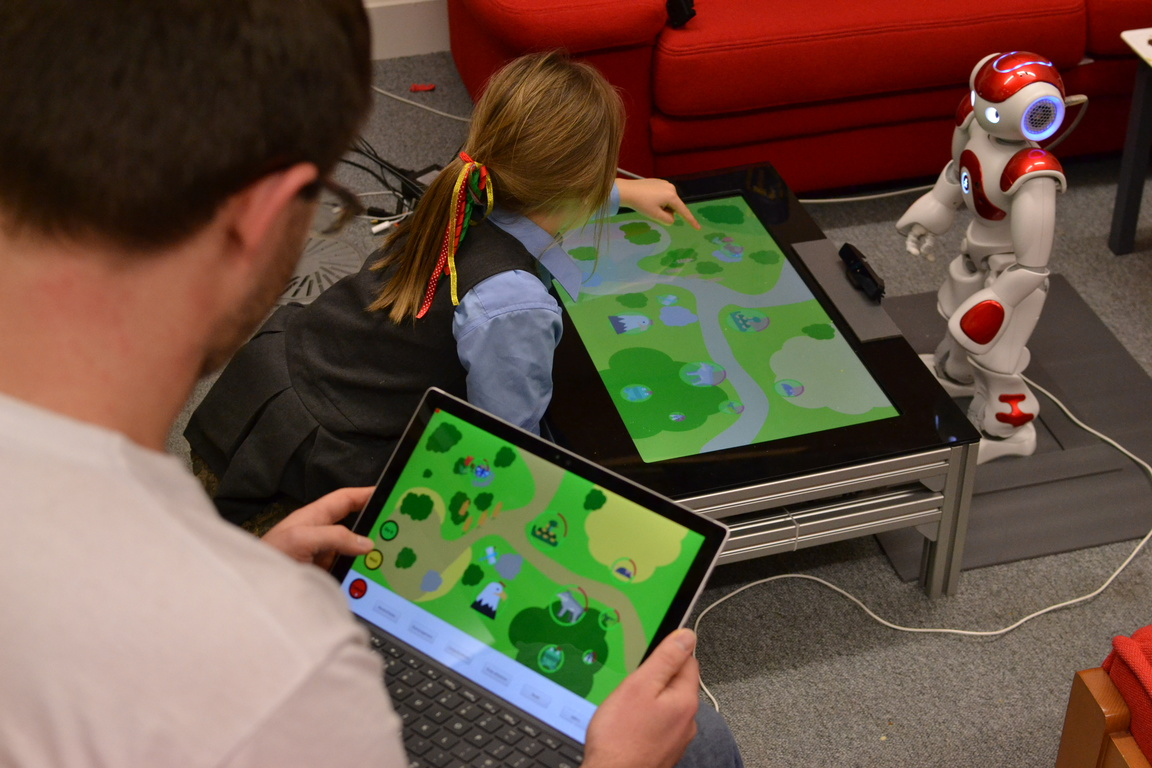
\includegraphics[width=.5\textwidth]{setup.jpg}
	\caption{Setup used in the study: a child interacts with the robot tutor, with a large touchscreen sitting between them displaying the learning activity; a human teacher provides supervision to the robot through a tablet and monitors the robot learning.}
	\label{fig:tutoring_setup}
\end{figure}

By interacting with the robot and the sandtray, the child is expected to gain knowledge on a specific topic. For this study, the task is learning about food chains by exploring a specific food web (interconnections between multiple food chains) in an educative game. The child plays a game on the sandtray where they can move animals to discover the interactions between them. Learning is evaluated by a test before, after and between the sessions; and the robot guides the child through the study and can, depending of the condition, support them during the game.

\subsection{Food Chain Game}

The main learning activity to teach the child the food web is a game composed of ten animals and three types of plants. Animals have energy decreasing over time and they have to eat to stay healthy. Animals are not moving unless the child or the robot moves them and can eat or be eaten when entering in contact with another animal or a plant. The child has to feed the animals by moving them to their food to give them more energy and by feeding the animals, children can learn what food each animal eats. Figure \ref{fig:tutoring_game} presents an example of the game screen in the middle of a session.

\begin{figure}[ht]
	\centering
		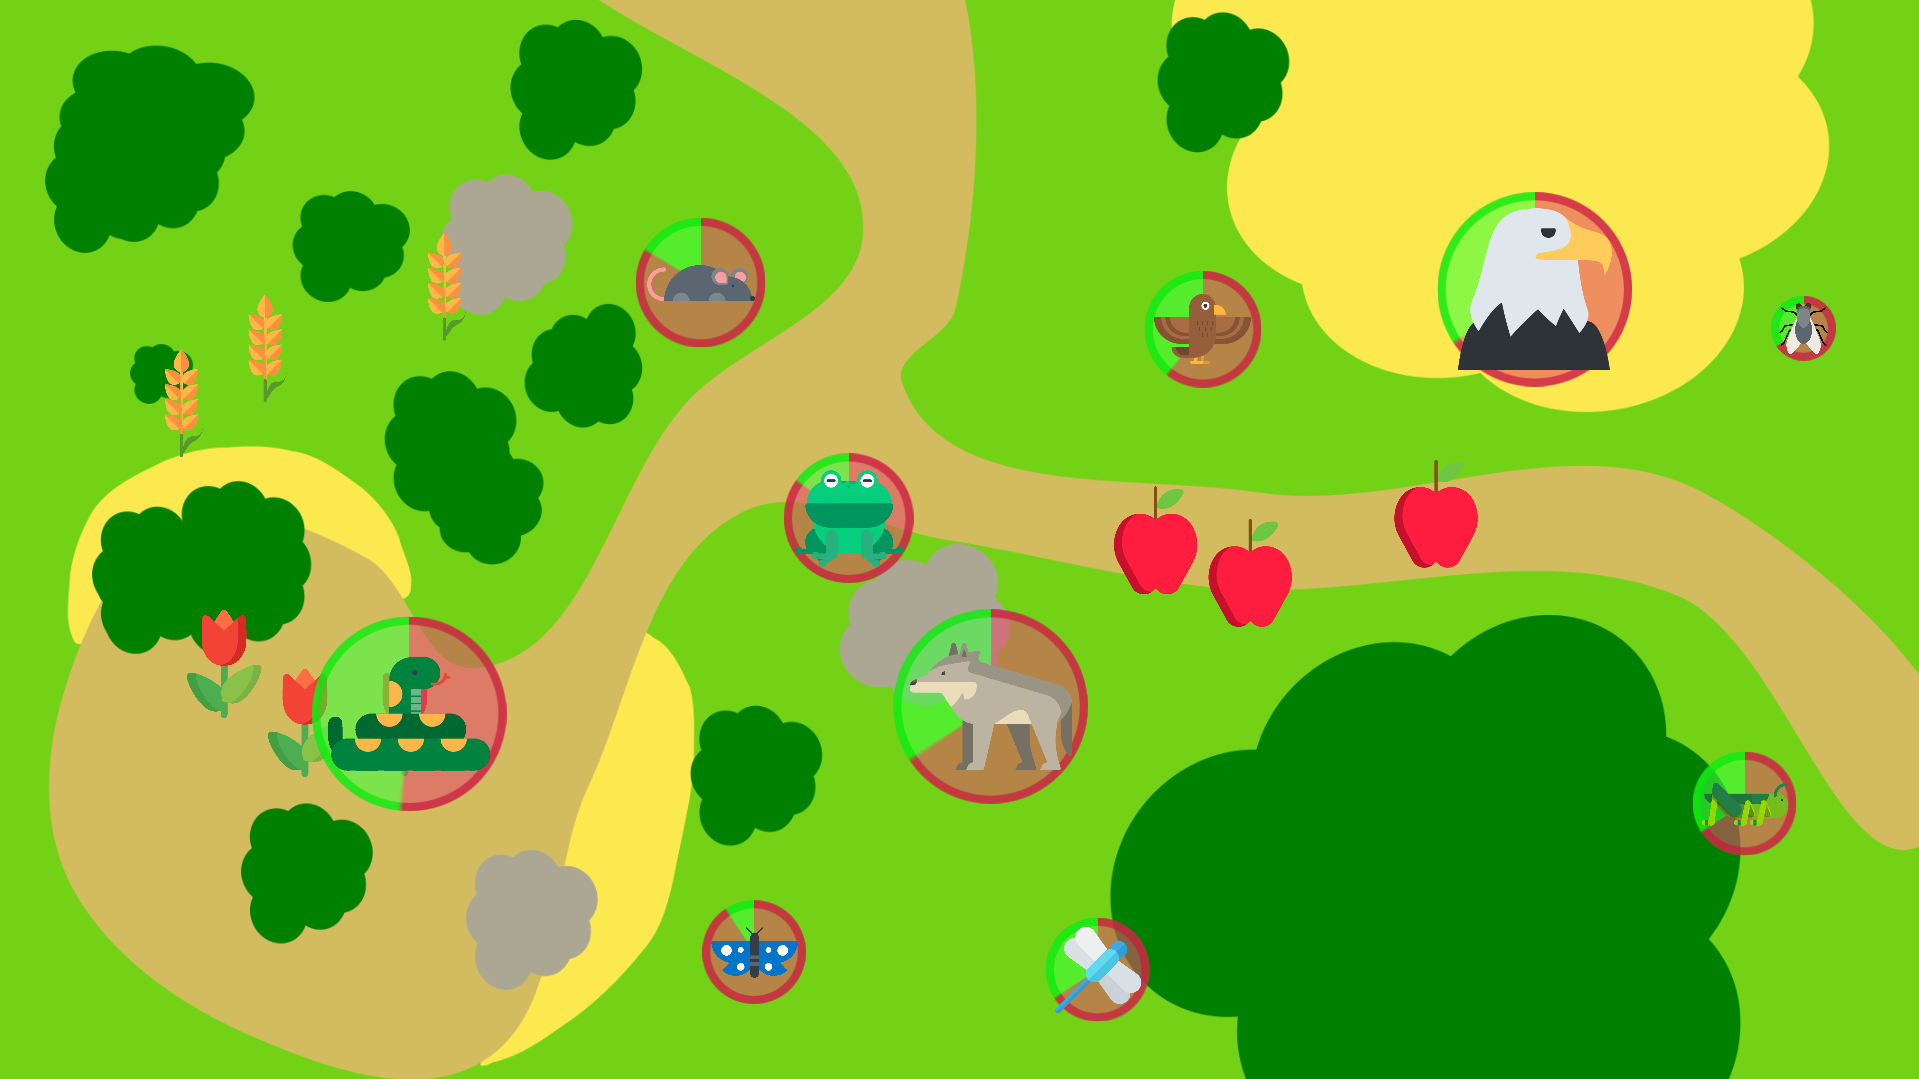
\includegraphics[width=1\textwidth]{game.png}
		\captionsetup{width=.9\linewidth}
		\caption{Example of the game. Animals have energy in green and have to eat plants or other animals to survive.}
		\label{fig:tutoring_game}
\end{figure}

\subsection{Robot Behaviour}
 
During the game, the robot can execute actions to provide hints and support to the child. The robot has access to five types of actions:
\begin{itemize}
	\item Movements: moving any animal to, toward or away from any items (animal or plant) - the robot points to an animal and moves it on the game while describing its action (e.g. "The eagle needs help getting close to the mouse").
	\item Drawing attention: the robot points an item and says a reminder to the child (e.g. "Don't forget the frog").
	\item Reminding rules: the robot says one of 5 sentences on the game (e.g. "Move the animals to feed them" or "Don't feed animals with a lot of energy").
	\item Congratulation: the robot provides congratulations (e.g. "Well done").
	\item Encouragement: the robot provides encouragement (e.g. "You can do it").
\end{itemize}
Considering all the possible combinations of actions and items, the total number of actions adds up 655. Additionally, to prevent the robot's behaviour to be repetitive and annoying, each utterance joining an action has multiple versions, and a random one not used recently is selected. 

This set of actions has been selected to be generalisable to many type of scenario including a teaching activity on a screen. Furthermore, in this study, these actions represent different level of support, from general motivation and information on the game's goal to which animals the child should focus on or direct information about what an animal eat. This selection of actions aims to cover a large range of possible tutoring behaviours humans could use. 

\subsection{Wizard of Oz Application}

In this study, the interface between the teacher and the robot occurs through the \gls{woz} application, a \gls{gui} running on a tablet and allowing the teacher and the robot to communicate. This \gls{gui} represents the state of the game as the child sees it, but with additional button and functionalities to communicate both ways with the robot (see Figure \ref{fig:tutoring_gui}). The teacher can use a combination of buttons and moving animals on the tablet to have the robot execute any possible action. For example, to move animals close to another item, the teacher can drag and release the animal's image to a position to request the robot to execute this movement. The robot controller will infer which action has been selected by the teacher by evaluating how the distances between animals changes. Additionally, the teacher can select other animals or plants to clarify their action and give information about what features were relevant in the decision process. Similarly, the teacher can select an animal and press the `Draw attention' button to have the robot point at the select animal and remind the child to use it.
%The main aim of the study being testing \gls{sparc} in a real \gls{hri}, the teacher needs an interface to communicate with the robot. To allow this interaction between the teacher and the robot, a \gls{gui} running on a tablet has been developed representing the current state of the game exactly as the child sees it on the touchscreen (see in Figure \ref{fig:tutoring_gui}). This \gls{gui} runs on a tablet as it allow the robot's teacher to supervise and teach the robot while monitoring the application interaction (i.e. the interaction between the child and the robot). Buttons for the actions (excluding movements) allow the teacher to select which action the want the robot to execute. The teacher can also have the robot move animals simply by dragging and releasing animals' images on the tablet. The teacher can also select animals or plants to specify which action they intend to do. 
For instance, by clicking on the frog and the `Draw attention' button, the robot will execute the \textit{drawing attention to the frog}. 
%Similarly, the moving action require two items: the animal moved and the target of the motion. By selecting a target before moving an animal, the teacher can be sure that the robot interpret the action correctly. 
This \gls{gui} design gives access to the teacher to the full 655 actions without requiring as many buttons. %Additionally, the selection of items is used by the robot controller to identify the relevant features to transmit to the algorithm for the learning.


\begin{figure}[ht]
	\centering
	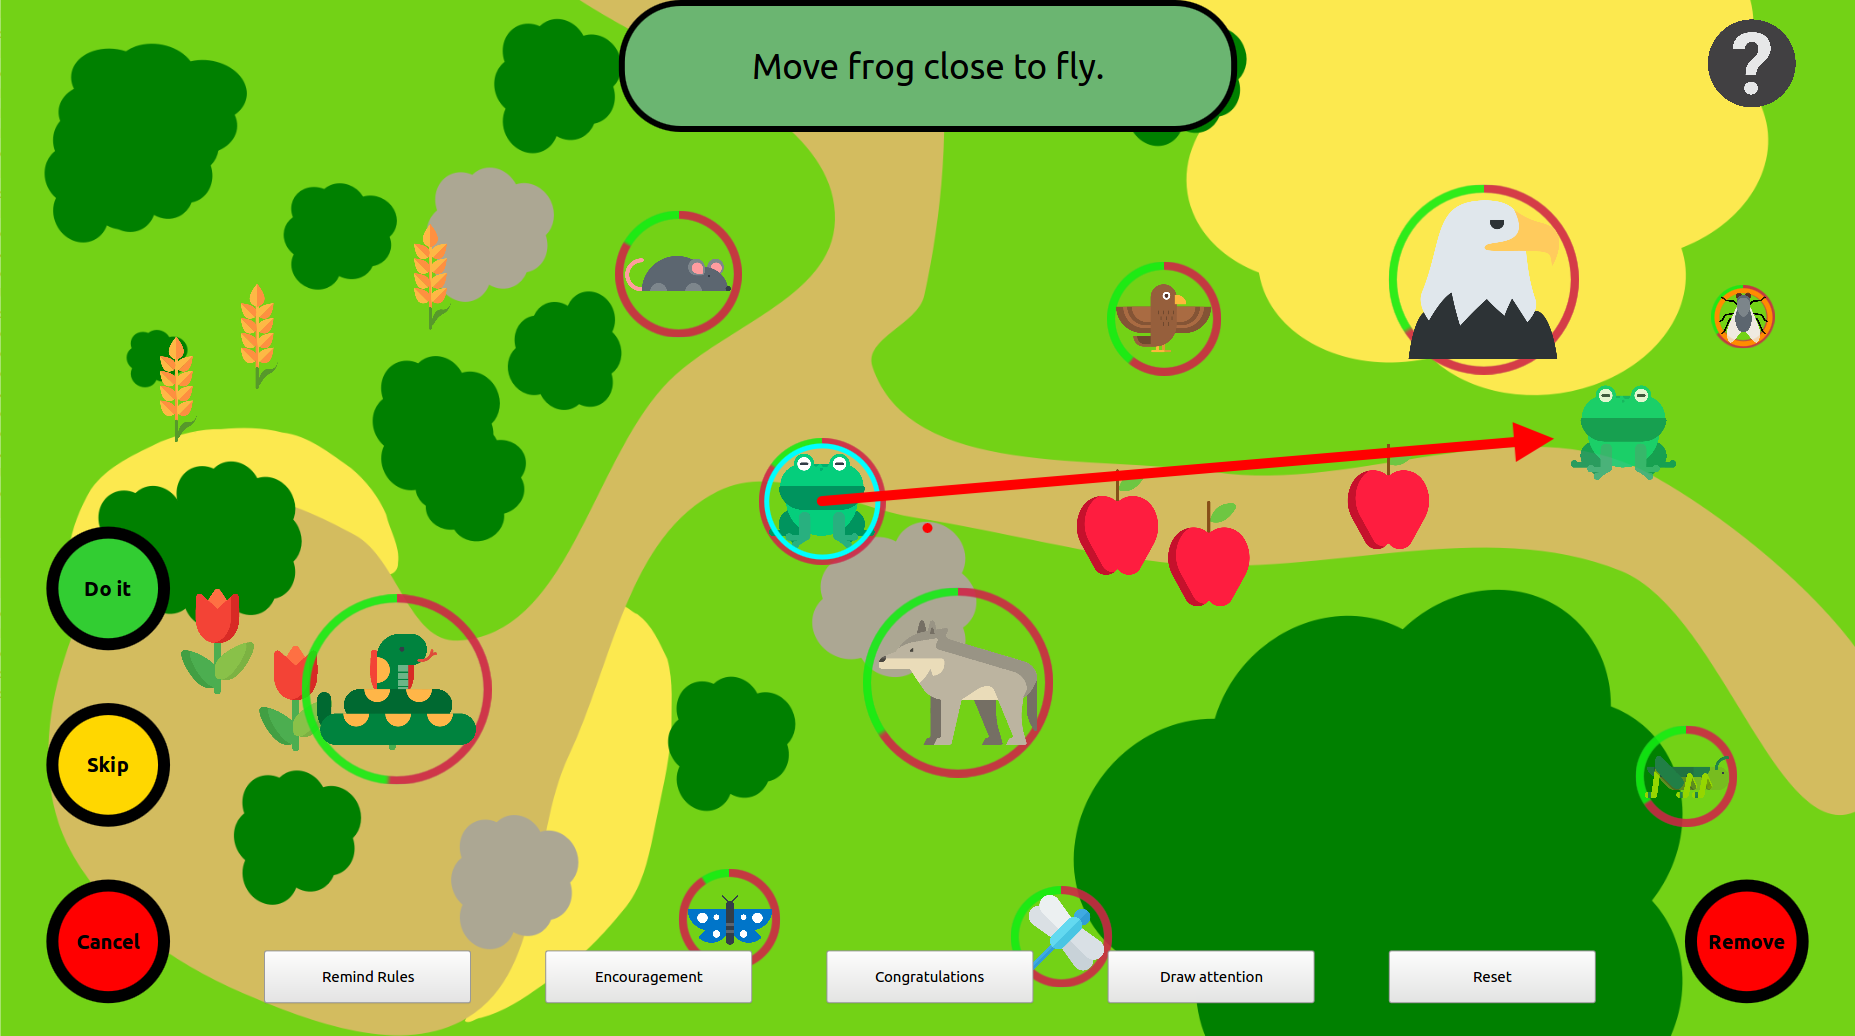
\includegraphics[width=1\textwidth]{gui.png}
	\captionsetup{width=.9\linewidth}
	\caption{\gls{gui} used by the teacher to control the robot and respond to its suggestions. The game is in the same state as in Figure \ref{fig:tutoring_game}, and he robot proposes to move the frog close to the fly (text bubble, arrow, moving the \textit{shadow} of the frog and highlight the frog and the fly).}
	\label{fig:tutoring_gui}
\end{figure}


Finally, the \gls{gui} is also used by the teacher to respond to the robot's propositions. Following the proposition of an action, a bubble describing the action will appear on top of the \gls{gui}, the corresponding items will be highlighted and if the action is a motion, an arrow will show the proposed motion. The teacher can react to the proposed action by pressing the `Do it', `Skip', `Cancel' or `Remove' buttons or let the action be executed. The action will be automatically executed after 2 seconds, during which the bubble will become greener to represent the passive acceptance of the action. The `Do it' button executes the action straight-away, the `Skip' button informs the algorithm that it should wait rather than doing the action, the `Cancel' button assigns a negative reward to this action in that state and finally, the `Remove' button looks for the closest previous instantiation of the action in memory and removes it, preventing this instance to be used later action selection.

\subsection{Algorithm}

The learning algorithm aims to reproduce the action policy by mapping an action (or no action) to each possible state. The state used in this study represents the situation of the game in a 210 dimensional vector, with value from 0 to 1. The dimensions include: distance between items, items' energy, time since events (child and robot touching each animal, robot's actions, interaction events: feeding an animal, death of an animal...), progression in the game sessions and child face direction (toward the robot, the screen or away). As mentioned before, the action space covers moving items in relation to other items, drawing attention to items, providing encouragements, congratulations and reminding the rules. In summary, the algorithm's task is to map an action from the 655 (including a `wait' action) to each possible combination on the 210-dimension state.

The actions and the state dimensions have been selected to be generic to many teaching tasks involving movable items: each item has a value assigned to it (here energy, but this could be changed in other scenario), and some movable items (here animals) can be move to, toward or away from other items. Using these generic actions and this state definition, this implementation could be easily re-purposed to another teaching task.

The algorithm used for the learning is an adaptation of the one presented in \cite{senft2017toward}. It is an instance based algorithm similar to the nearest-neighbours algorithm \cite{cover1967nearest}. However, two differences are notable compared to the initial algorithm. %: instances are defined on a sliced part of the state and each instance instance is associated to a reward defining the interest of the agent to select this action in that state.
Firstly, instead of being defined on the full state space, instances are defined on a sliced version of the state. The intuition is that states needed to cover complex action policies require large number of dimensions, however for each single action, large parts of the state are irrelevant. For example, if a robot needs to pick-up a cup, the colour of the cup does not impact the optimal motion. In contrast, the colour matters if the robot has to answer the question: ``which cup is on the left? The blue one or the red one?''. Consequently, the colour of the cup should be part of the state space, but should not be considered when selecting some of the actions. For this implementation, when selecting actions, the teacher can highlight features of the environment which \emph{activates} specific dimensions of the state space which are used to store the instance in memory. By default, all the generic events (death, feeding, failed interaction) were \emph{activated}. All the \emph{non-activated} dimensions are left as wild-cards. Then, when comparing the current state to the saved instances, the distance is only computed on the \emph{activated} dimensions of the stored instance. The second difference is that each instance saved has a reward assigned to it. For this study, if the teacher selects the action, the \gls{gui} assigns a reward of $+1$, and if the teacher cancels the action (following an incorrect suggestion from the algorithm) the reward is $-1$. When selecting an action, the algorithm looks through all the actions it has been using and for each action selects the closest instance to the current state and computes the expected reward as a multiplication of the distance by the reward. Then the algorithm selects the action with the highest expected reward and proposes it if the value is higher than an adaptive threshold. 

The algorithm runs at 2Hz while we would expect actions to be selected every 5 to 20 seconds. So, unlike most of the discrete cases of action selections, in most of the steps no actions are required. To handle this difference of timescale, a waiting action have been added (through the `Skip' button) and an adaptive threshold limits the propositions to actions with a high expected reward. Selecting an action can reduce the threshold, and cancelling or skipping an action can increase it. This aims to adapt the rate of action propositions to the desires of the teacher. A last mechanism filters propositions from the algorithm not to transfer them to the teacher when an action is already proposed or the robot is currently acting. This filter also rewards negatively impossible actions (such as moving dead animals).

\subsection{Study Design}

%Parents completed a consent form and each child was proposed to withdraw if they appeared not interested to continue the study (children refusing to continue have been replaced to reach the same number in each category). 
The interaction protocol was as follows. Children were first introduced to the robot and the aim of the interaction and then had a first pre-test to evaluate their initial knowledge. Before starting the teaching game, children had to complete a tutorial where they were introduced to the mechanics of the game: animals have life and have to eat to survive and children can move animals to make them interact with other animals or plants and replenish their energy. After this short tutorial, they completed two sessions of the game where the robot could provide feedback and advices depending on the conditions they were in. Following these initial sessions of the game, children completed a mid-test before playing another 2 sessions of the game and a last post-test to conclude the study. 

%\begin{figure}[h]
%	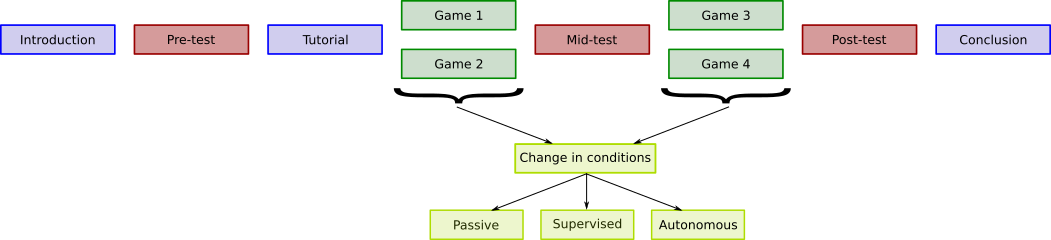
\includegraphics[width=.9\linewidth]{graph.png}
%	\centering
%	\caption{Methodology used for the study.}
%	\label{fig:method}
%\end{figure}

The study evaluated three conditions: the passive condition, supervised condition and autonomous condition. In all the conditions, the robot's behaviour during the introduction, tests, tutorial and conclusion was identical. The only change of behaviour happened during the games sessions. As the study design is between participants, children were each assigned to a condition, and in all the game session, the robot would be passive, supervised or autonomous. %In the passive condition, the robot does not provide support during the game. In the supervised condition, the robot is controlled by a PhD student in psychology acting as the robot's teacher and demonstrating it how to interact. And in the autonomous condition, the robot simply applies the learned policy without supervision.

In the \textit{Passive} condition, the robot does not provide any advice nor feedback to the children during the game sessions. It only oscillates slightly to simulate a breathing motion and follows the child's face. In the \textit{Supervised} condition, the robot is remotely supervised by an operator using \gls{sparc}. Finally, in the \textit{Autonomous} condition, the robot applies the learnt policy and provides feedback and guidance to the child without human supervision.

In the study, the teacher was a psychology PhD student from the university, with limited knowledge in computing and machine learning. She has been instructed how to control the robot using the GUI, the effect of each buttons and how to perform each action. She was knowledgeable of the methodology used to run the study (but not the underlying implementation) and experimented controlling the robot in two interactions with the author interacting with the robot and one with a child before starting to supervise the robot for the supervised condition. No information about the learning algorithm or the representation of the state and no feedback about optimal way of interacting or feedback on her action policy was provided before or during the supervision. As such, this robot teacher represents typical target populations for robotic applications: non-experts in machine learning or computing but with relevant domain knowledge such as teachers or psychologists.

In the \textit{Autonomous} condition, the robot uses the suggestions from the algorithm and executes them with a probabilistic delay between 0 and 1.5 seconds based on the teacher's delay in answering the robot's propositions. This delay aims to give a pace and synchronisation of actions similar to the ones exhibited by the teacher when reacting to the robot's suggestion.

% Figure \ref{fig:tutoring_game} shows an example of the game screen. The child can move 10 animals across the game field and can have them interact with other animals or plants. Animals lose energy over time and by interacting with their food the can regain some. Animals that are eaten lose a chunk of their life. The goal for the children is to keep animals alive as long as possible by feeding them and they earn stars representing how healthy their animals have been during the session. The game stops when 3 or more animals run out of energy and each game session lasted 1.6 minutes in average.

\subsection{Metrics}

%Redundant with hypothese?
%This study aimed mostly at evaluating if \gls{sparc} allows a human non-expert in computing to teach a robot from in-situ supervision. 
%This teaching capability is divided into three parts: 
%\begin{itemize}
%	\item How similar the teacher's and autonomous robot's policies are? 
%	\item What are the impacts of the active robot on the child behaviour? \\(And what are the differences between the autonomous and supervised robots?)
%	\item How the online learning component changed the interaction between the robot and the teacher?
%\end{itemize}

To address the hypotheses presented in Section \ref{sec:tutoring_scope}, we collected multiple metrics on both interactions (teaching and application) and on the child performance. First, we recorded the actions executed by the robot in the supervised and autonomous conditions to characterise their action policies. Two groups of metrics have been collected for evaluating the application interaction: the learning metrics (corresponding to children's performance during the test) and the game metrics (corresponding to children's behaviour during the game). And finally, in the supervised condition, we recorded the origin of the action executed by the robot (teacher vs algorithm) and the outcome of the proposed actions (executed vs refused).

\subsubsection{Policy Characterisation}

During the game, the robot has access to 622 actions, which can be divided in seven categories: drawing attention, moving close, moving away, moving to, congatulation, encouragements and reminding rules. Due to this high number of actions, the largeness of the state space (210 dimension) and the complex interdependence between actions and states, totally defining a policy is impossible. Consequently, we propose to use the number of actions executed per child for each category to characterise the policy executed by the robot in the active conditions (supervised and autonomous). While not perfectly representing the action policy of each condition (e.g. the timing of actions is missing), this metric offers a proxy to compare these policies. 

\subsubsection{Learning Evaluation}
During the pre-test, the experimenter demonstrated how to connect animals by drawing an arrow from the frog to the fly, and then removing the arrow by pressing the \textit{X} button. Then, children were asked to connect as many animals as possible. Figure \ref{fig:test} shows two examples of the test, with or without all the correct connections. When children thought they were done, they could press the `Continue' button, showing a screen asking confirmation to quit the test or allowing children to keep connecting animals. Additionally, the robot informed the child if not all the animals were connected to a food or that animals could eat many types of food if no more than one animal was connected to two items. 

\begin{figure*}[ht]
	\centering
	\begin{subfigure}[t]{0.5\textwidth}
		\centering
		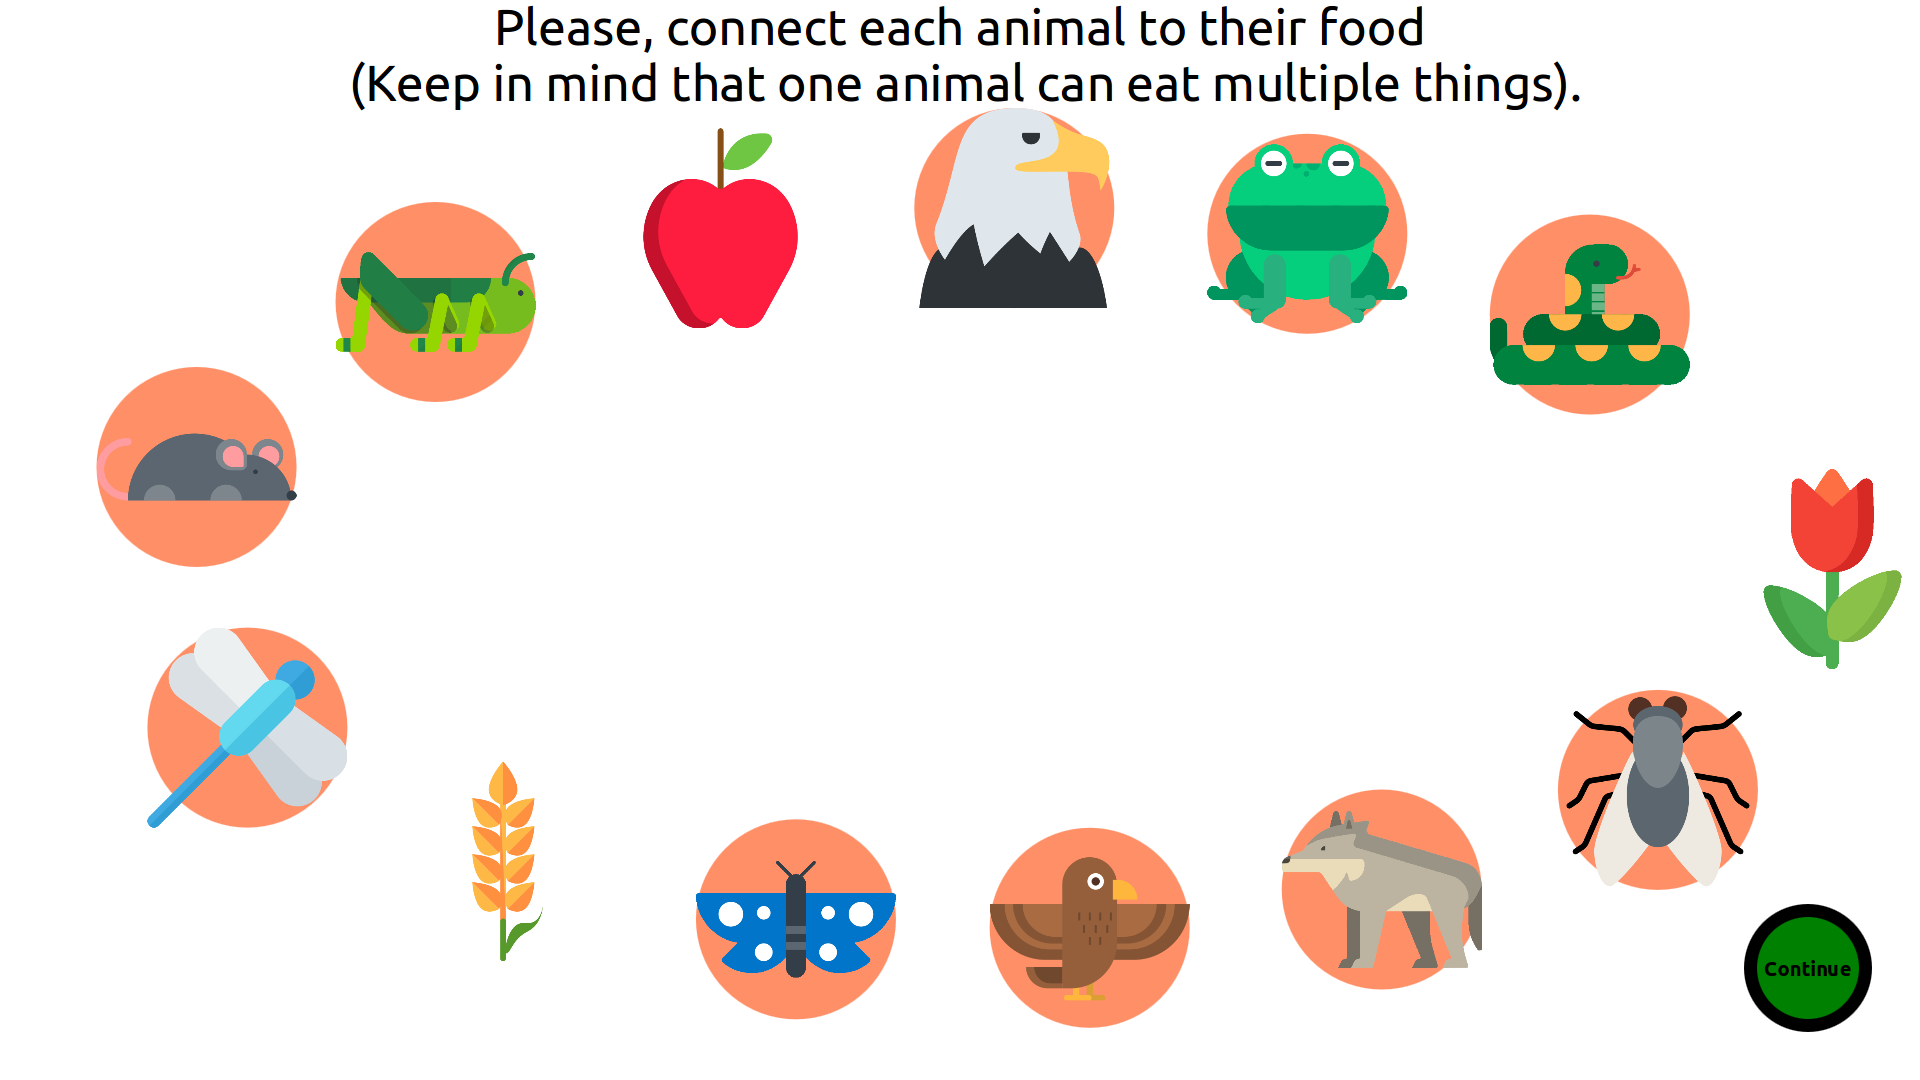
\includegraphics[width=0.95\textwidth]{empty_graph.png}
		\captionsetup{width=.95\linewidth}
		\caption{Empty screen that children face at each test. Red dots behind animals represent that they are not been connected to any food.}
	\end{subfigure}%
	~ 
	\begin{subfigure}[t]{0.5\textwidth}
		\centering
		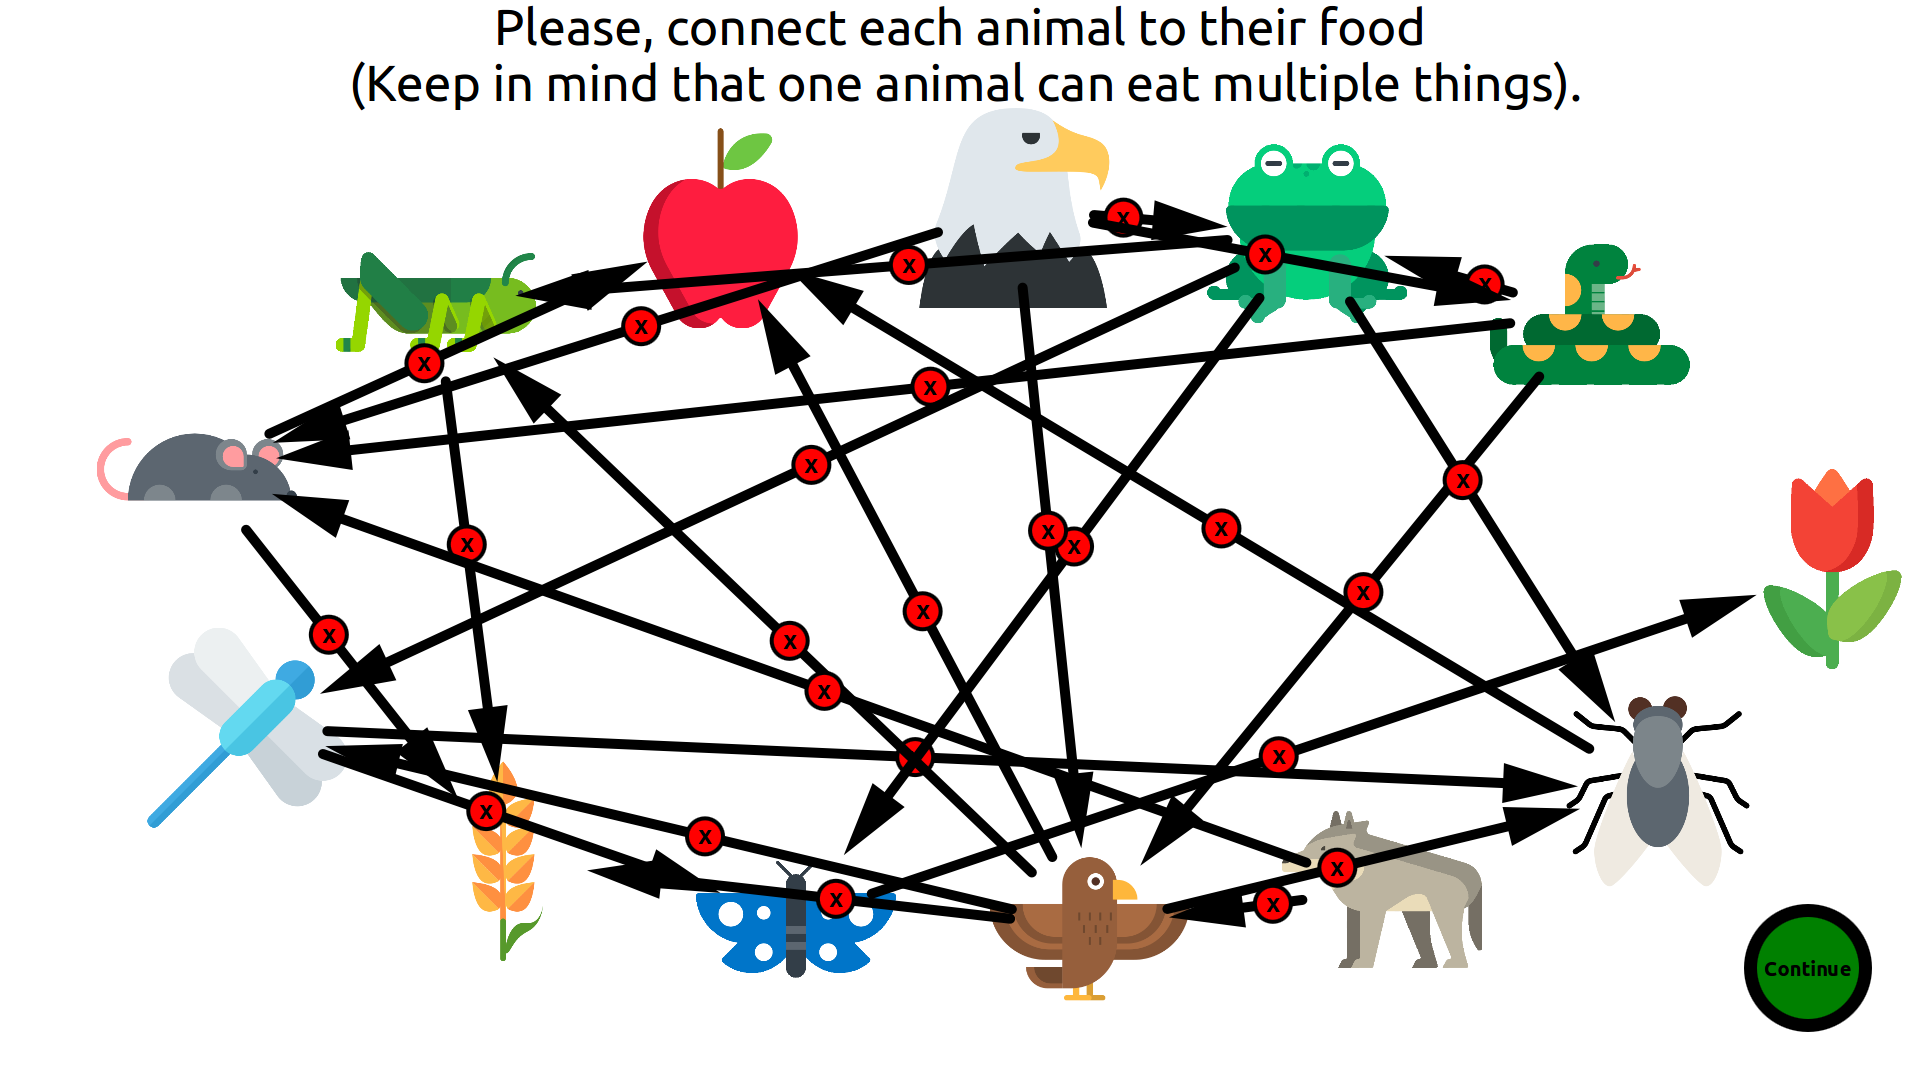
\includegraphics[width=0.95\textwidth]{full_graph.png}
		\captionsetup{width=.95\linewidth}
		\caption{Fully connected test with all the correct connections.}
	\end{subfigure}
	\caption{Test screen to evaluate children's knowledge, empty starting screen (a) and fully connected and correct test (b).}
	\label{fig:test}
\end{figure*}

They are in total 25 different correct connections and 95 possible incorrect ones. As the child can connect as many arrows as desired, the performance is defined as the number of correct arrows above chance (for the number of connected arrows on the test) divided by the maximum achievable performance to reach a score bounded to $[-1,1]$. For example, if a child connects 5 good arrows and 3 bad, their performance would be:

\begin{equation}
P=\frac{\#good-(\#good+\#bad) \cdot \frac{total good}{total}}{total good - total good \cdot \frac{total good}{total}} = \frac{5-(5+3) \cdot \frac{25}{25+95})}{25 - 25 \cdot \frac{25}{25+95}}=0.168
\end{equation}
			
The three tests (pre, mid and post interaction) result in three performance measures. To account with initial differences of knowledge and the progressive difficulty to gain additional knowledge, we computed the learning gain as the difference between the final and initial knowledge divided by the `progression margin': the difference between the maximum achievable performance and the initial performance. This learning gain indicates how much of the missing knowledge the child managed to gain from the game.
			
\subsubsection{Game Metrics}

Different metrics have been gathered during the game sessions to characterise the children's behaviours:
\begin{itemize}
	\item \textbf{Interaction time}: Duration of game sessions, how long a game lasted until three animals ran out of energy.
	\item \textbf{Points}: cumulated sum of animals' energy over the game (typical range [550,1100]).
	\item \textbf{Number of different eating interactions}: number of unique feeding action type.
\end{itemize}

Both the interaction time and the number of points reached in the game inform on the children's success for the task: keeping the animals alive as long as possible. The last metric: the number of different eating interactions informs on how many learning items the children have encountered in the games. A feeding interaction happens when an animal is moved to its food (or to a predator); and the number of different feeding interaction represents how many different correct connections the child has has been exposed during the game (multiple feeding actions between the same animals would count only once). A game with a high number of different feeding represents a game where the child had the opportunity to learn many correct connections between animals. Consequently, by increasing this number, the children would be exposed to more learning items which should help them to perform better on the tests. 

%Maybe talk about compliance

\subsubsection{Robot Learning}

In the supervised condition, the robot executes actions selected or validated by the teacher. By using \gls{sparc}, the robot can propose actions to the teacher. Faced with a proposition, the teacher has multiple ways to react. They can accept the action (by waiting for it to be executed, pressing `Do it' or selecting the same action manually) or refuse it by pressing the `Cancel', `Skip' or `Remove' buttons. Actions can be divided in three categories: actions selected by the supervisor,robot's good propositions and robot's bad propositions. And the evolution of these categories represent how much the online component of the learning improves the quality of the robot's suggestions and reduces the workload on the teacher. 

Some times the teacher cancelled actions and then selected them again, we called this effect the `reselection'. To obtain the final numbers of accepted and refused actions, we removed these reselection from the bad propositions and we added them to the good propositions as it represents cases where the teacher refused an action by accident.

\section{Results}

To demonstrate the presence or the absence of effects, we used bayesian statistics on the data. As such the Bayes factor $B$ is reported and represents how much of the variance on the metric is explained by a parameter (if $B < 1/3$ there is no impact, if $B > 3$ the impact is strong, and if $1/3<B<3$ the results are inconclusive; \cite{jeffreys1998theory,dienes2011bayesian}). 

%Preliminary results (currently in progress, due to be completed before the submission of the full article) show that (1) the robot is able to effectively jointly learn action and social policies (Figure 2), (2) the learning gains of the children supported by the autonomous robot are not significantly different from the gains when the learning is supported by a robot tele-operated by the human expert, which would indicate the utility of the approach.

\subsection{Comparison of Policy}

Figure \ref{fig:tutoring_actions} presents the number of actions of each types executed by the teacher (in the supervised condition) and the autonomous robot. Both action policies present similarities: the action `Move away' is almost never used, `Move to' is never used, and the supportive feedback (`Congratulation' and `Encouragement') are used more often than `Remind rules' or `Drawing attention'. However, some dissimilarities are also present, for instance, the autonomous robot uses more encouragements than congratulations while the teacher did the opposite. The autonomous robot also reminded the rules more often and used the `Move close' action less than the supervisor. These differences of actions are linked to the type of machine learning used; with instance based learning, some datapoints will be used in the action selection much more often than others presenting some biases. But these results show that the robot managed to learn a social and technical action policy presenting similarities with the one displayed by the teacher providing partial support for H1.

\begin{figure}[ht]
	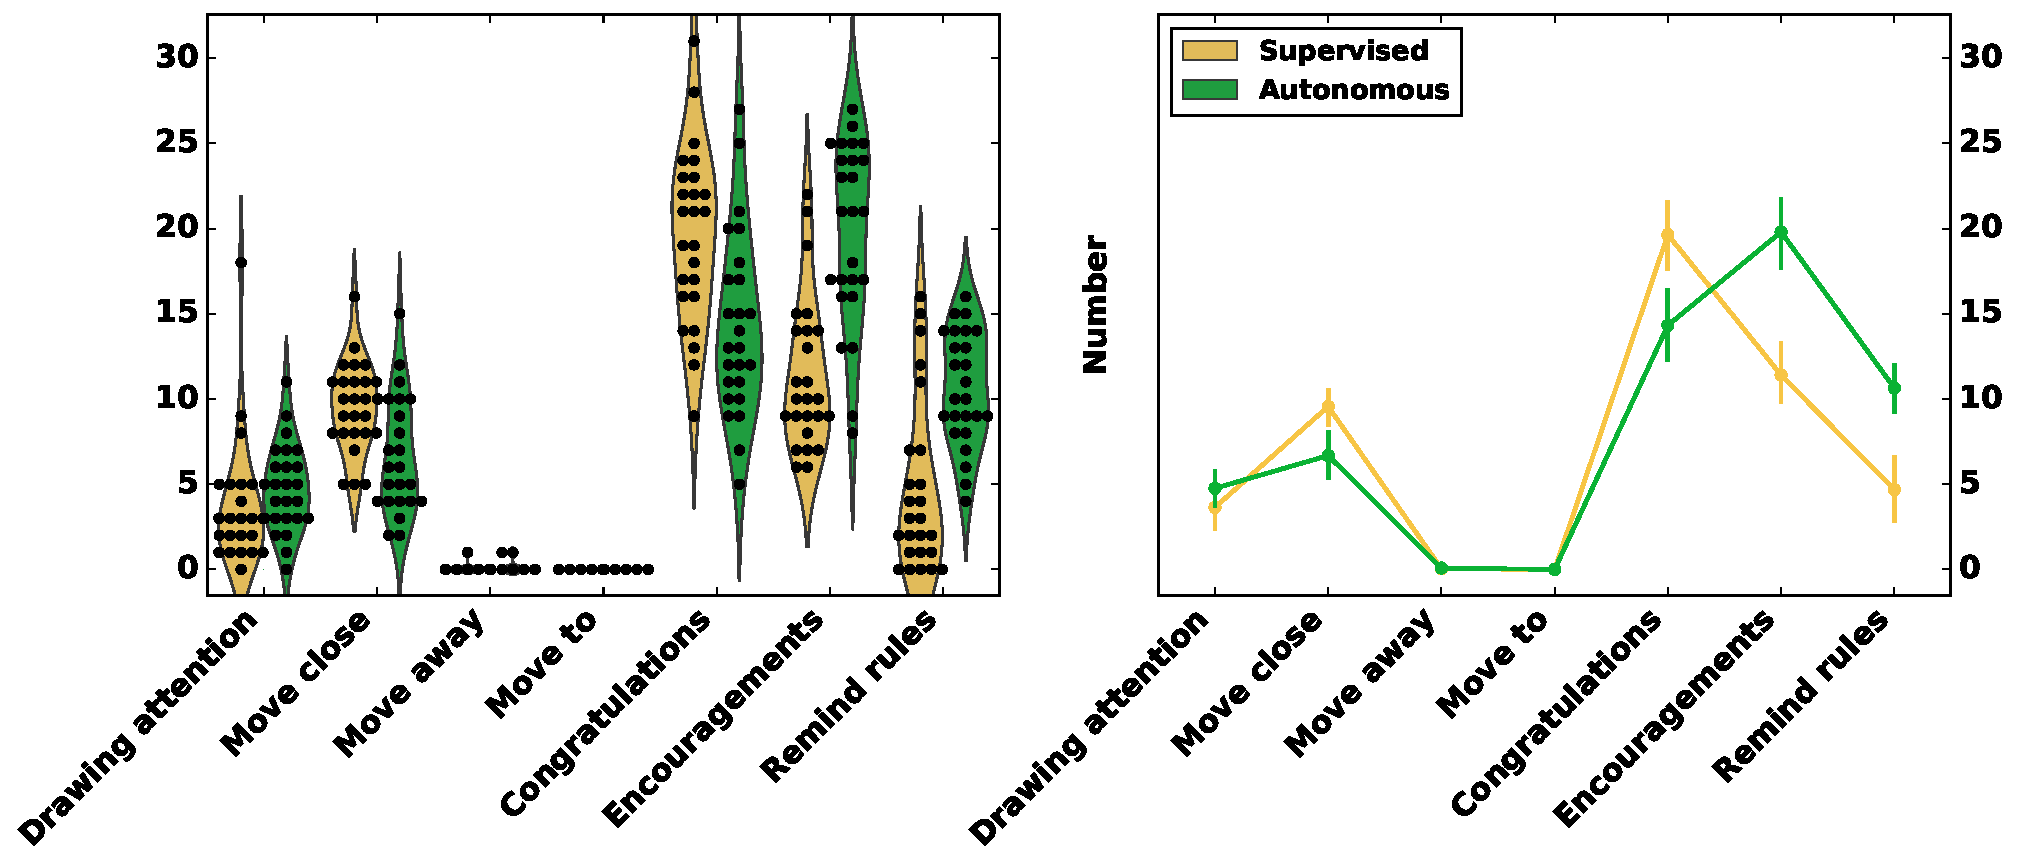
\includegraphics[width=1\linewidth]{actions.pdf}
	\centering
	\caption{Comparison of actions executed for the autonomous and supervised condition.}
	\label{fig:tutoring_actions}
\end{figure}


%\begin{figure}[ht]
%	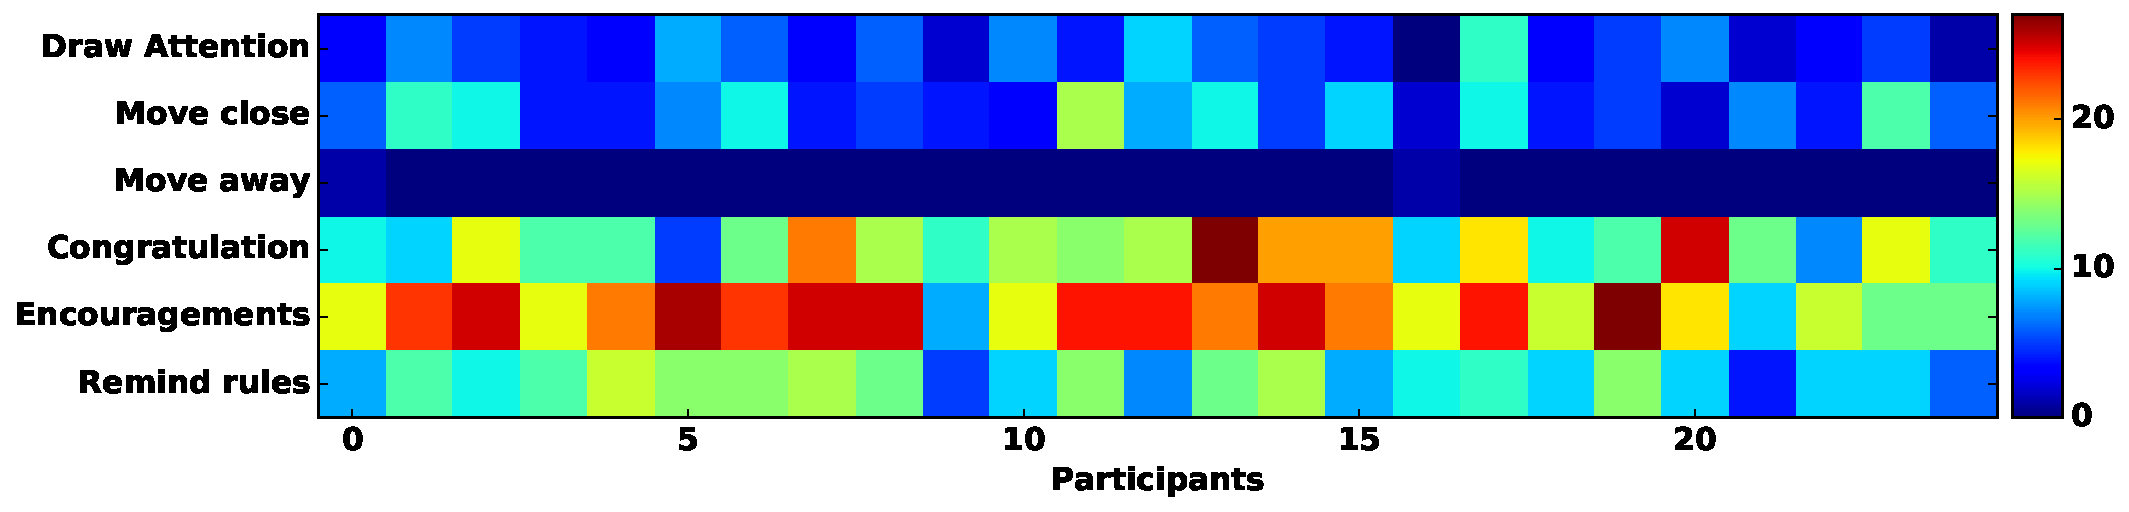
\includegraphics[width=1\linewidth]{autonomous_actions.pdf}
%	\centering
%	\caption{Repartition of actions across the participants in the autonomous condition.}
%	\label{fig:tutoring_autonomous_actions}
%\end{figure}
%
%\begin{table}[ht]
%	\centering
%	\caption{Repartition of action in the policy for both conditions (in \%).}
%	\label{tab:tutoring_policies}
%	\begin{tabularx}{\textwidth}{@{}lYYYccY}\toprule
%		& Draw \newline Attention & Move \newline close & Move \newline away & Congratulation & Encouragements & Remind \newline rules \\
%		\midrule
%		Supervised & 6.6  & 22.2 & 0.1 & 43.1 & 22.7 & 5.3 \\
%		Autonomous & 8.5 & 11.8 & 0.1 & 25.4 & 35.2 & 18.9\\
%		\bottomrule
%	\end{tabularx}
%\end{table}


\subsection{Test Performance}

Figure \ref{fig:tutoring_performance} shows the evolution of children's performance across the three tests. A Bayesian mixed-ANOVA show that in all conditions, children's performance increased across the tests ($B=1.5$x$10^{12}$), however the impact of the condition on the learning is inconclusive with a tendency to show no impact ($B=0.539$). This indicates that by being involved in the task, every children learned and improve their performances on the test (by gaining in average 13\% of the missing knowledge), but the robot behaviour during the game did not have an important impact on the children's learning gain (see Figure \ref{fig:tutoring_learning}), invalidating H2.

\begin{figure}[ht]
	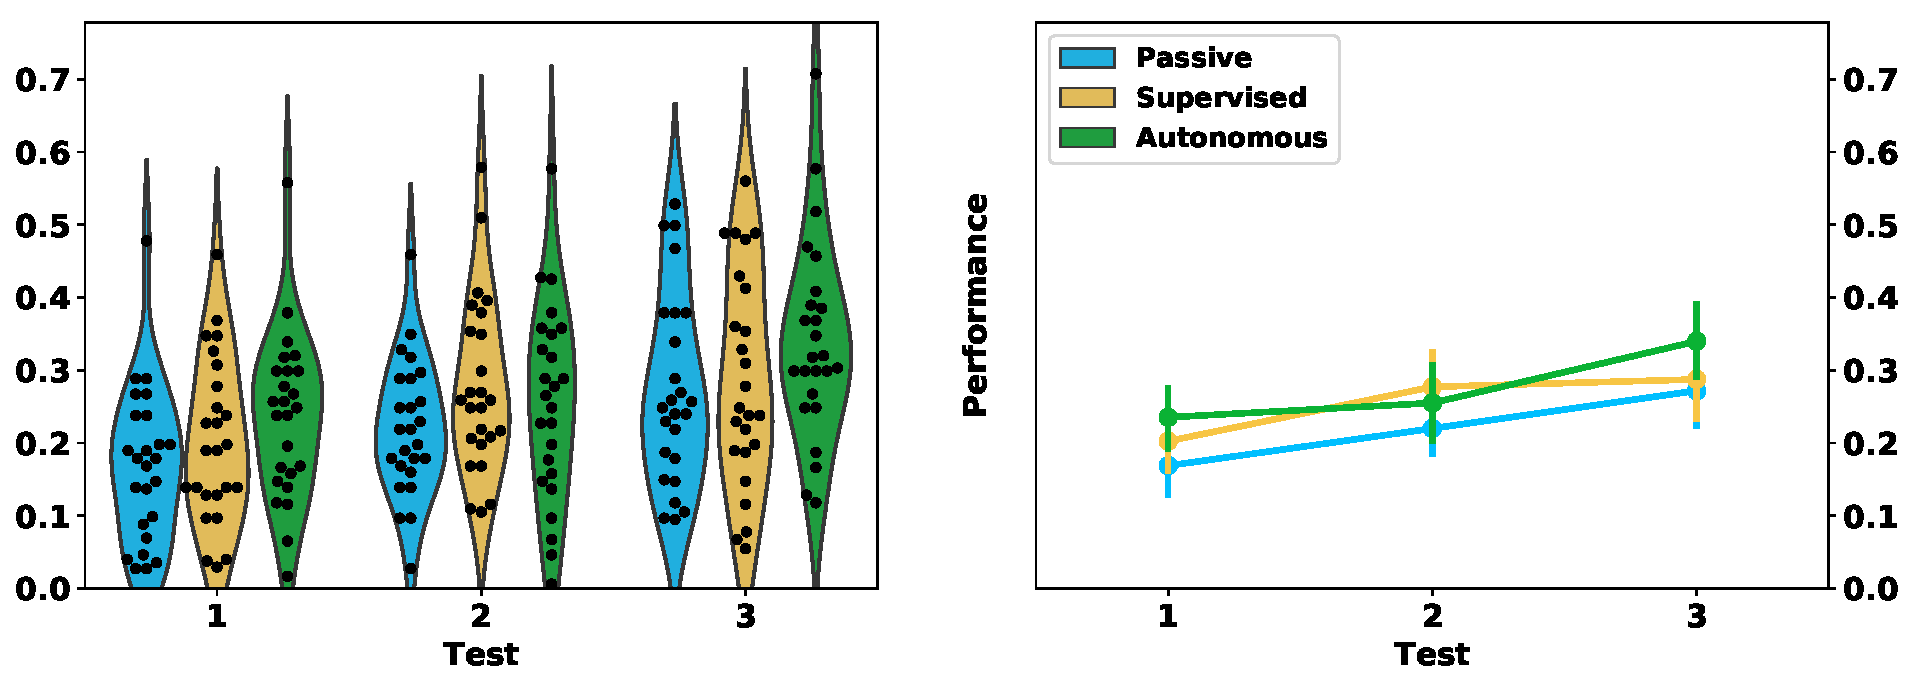
\includegraphics[width=1\linewidth]{perf.pdf}
	\centering
	\caption{Children's performance for the three tests: pretest, midtest and posttest for the three conditions.}
	\label{fig:tutoring_performance}
\end{figure}

\begin{figure}[ht]
	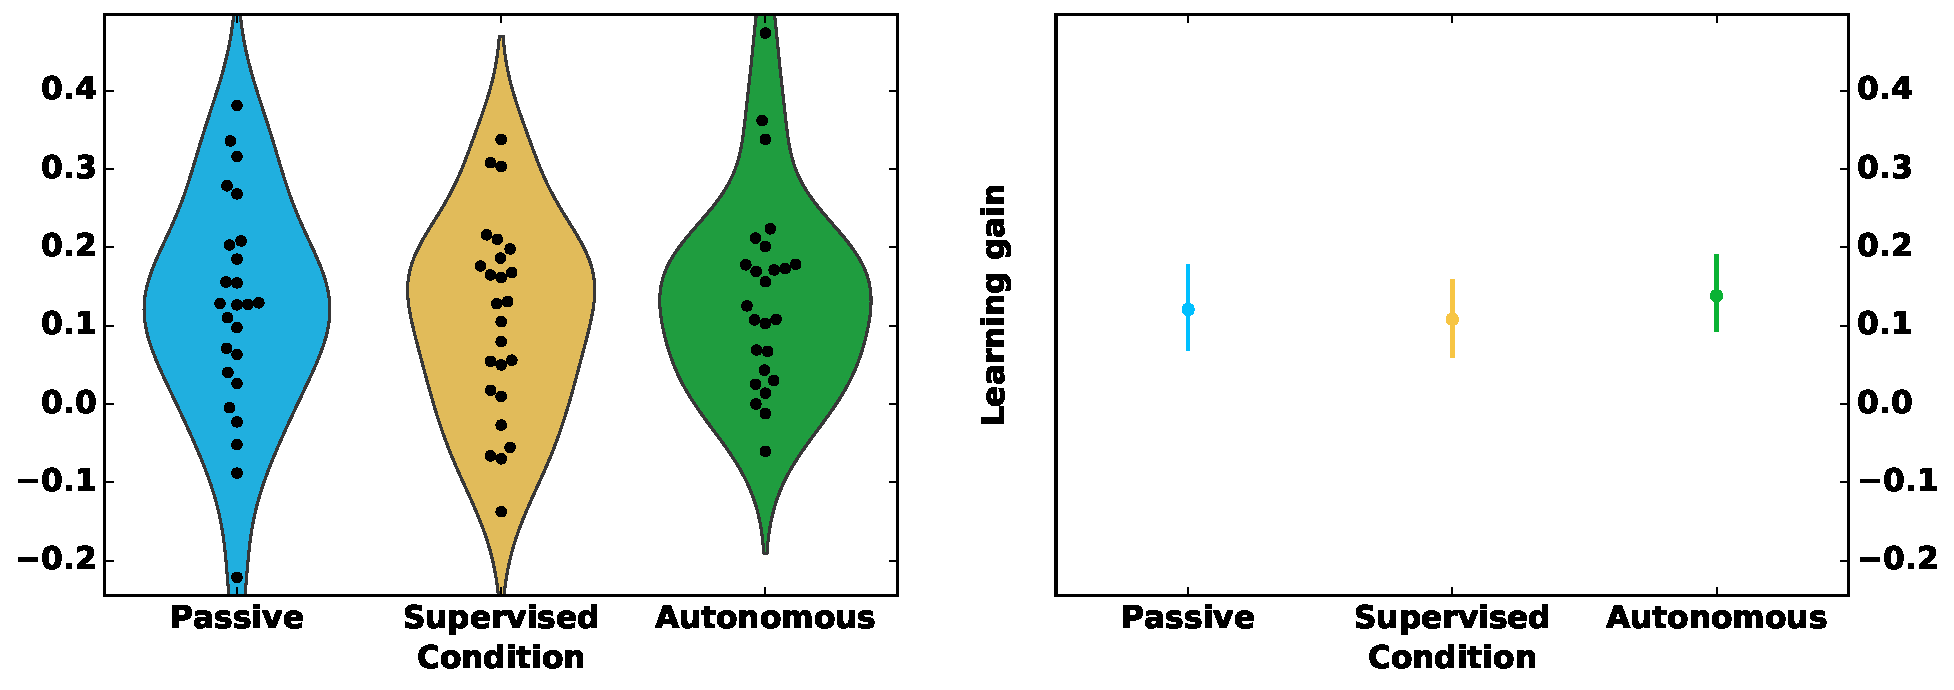
\includegraphics[width=1\linewidth]{learning.pdf}
	\centering
	\caption{Children's normalised learning gain after interacting with the robot for the three conditions.}
	\label{fig:tutoring_learning}
\end{figure}

\subsection{Game Metrics}

\paragraph{Different eating behaviours}

ES: I might rename it later, maybe something like exposure to learning items...

Figure \ref{fig:tutoring_d_eat} shows the evolution of the number of different eating behaviour exhibited by the children across the four game sessions. A Bayesian mixed-ANOVA shows an impact of the condition on the number of different eating behaviour produced by the children in the game ($B=6.1$). Post-hoc tests show that there is no difference between the Supervised and the Autonomous conditions ($B=0.154$), whilst differences are observed between the Supervised and the Passive condition ($B=512$) and between the Autonomous and the Passive conditions ($B=246$). This indicates that, compared to the Passive robot, the Supervised robot provided additional knowledge to the child during the game, allowing them to create more useful interactions between animals and their food, receiving more information from the game potentially helping them to learn. And the Autonomous robot managed to recreate autonomously this effect without the presence of a human providing input.

\begin{figure}[ht]
	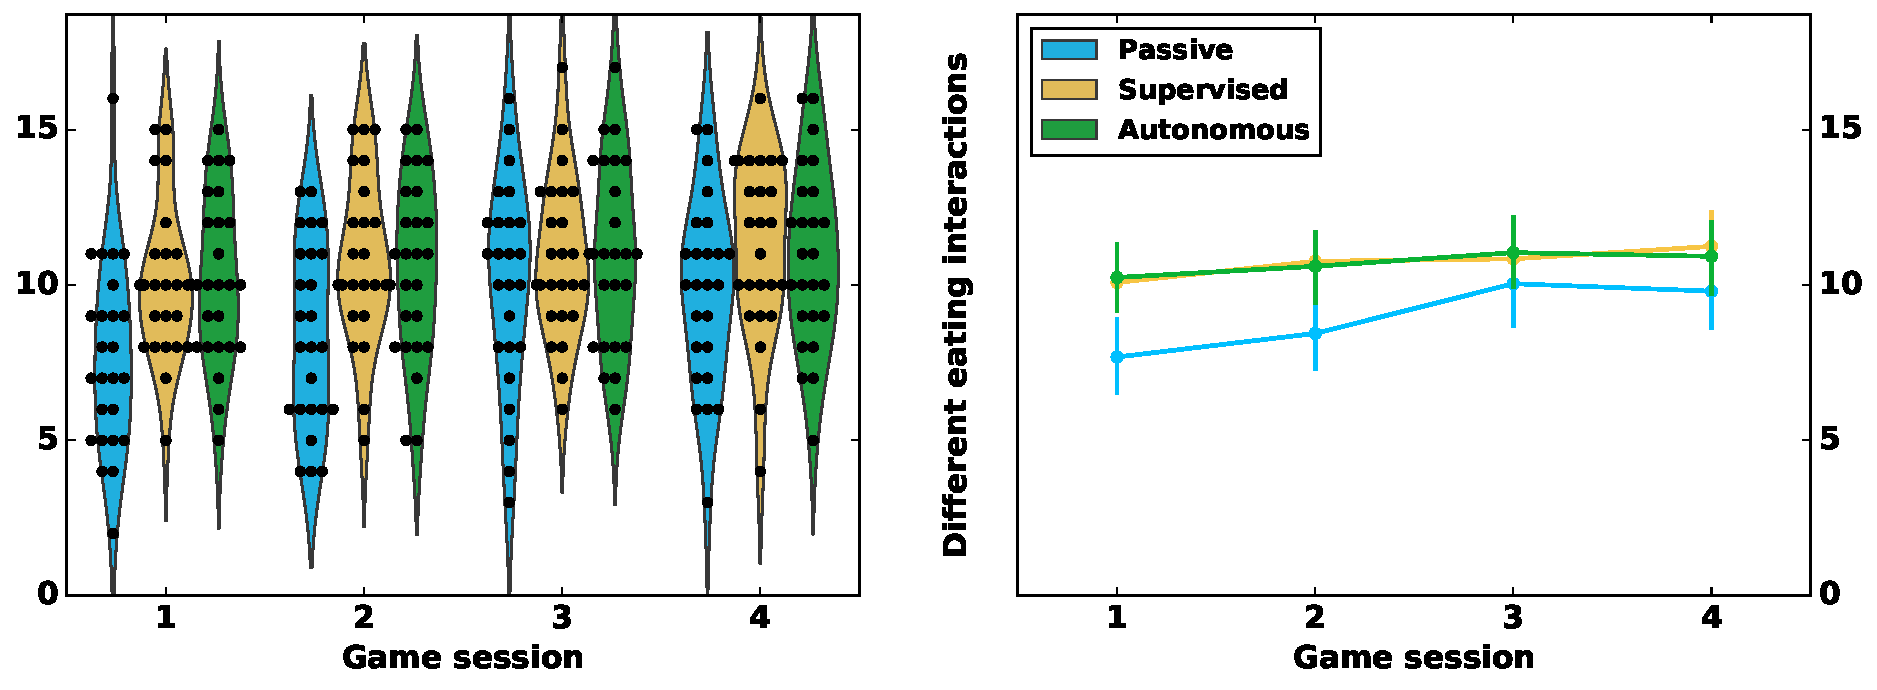
\includegraphics[width=1\linewidth]{d_eat.pdf}
	\centering
	\caption{Number of different eating behaviour for the four games for the three conditions.}
	\label{fig:tutoring_d_eat}
\end{figure}

\paragraph{Points}

Figure \ref{fig:tutoring_points} shows the evolution of the number of points achieved by the children across the four game sessions. A Bayesian mixed-ANOVA shows an impact of the condition on the number of points achieved by the children in the game ($B=10.2$). Post-hoc tests show a strong difference between the Passive and the Supervised conditions ($B=5.1$x$10^4$) and differences between the Supervised and the Autonomous conditions ($B=5.2$) and the Autonomous and the Passive condition ($B=5.9$). This indicates that when the robot was supervised, it allowed children to achieved more points than a  passive robot. And a similar effect is observed when the robot is autonomous, however the autonomous robot did not manage to reach the same efficiency as the supervised robot in helping the children to achieve a high score in the game.

\begin{figure}[ht]
	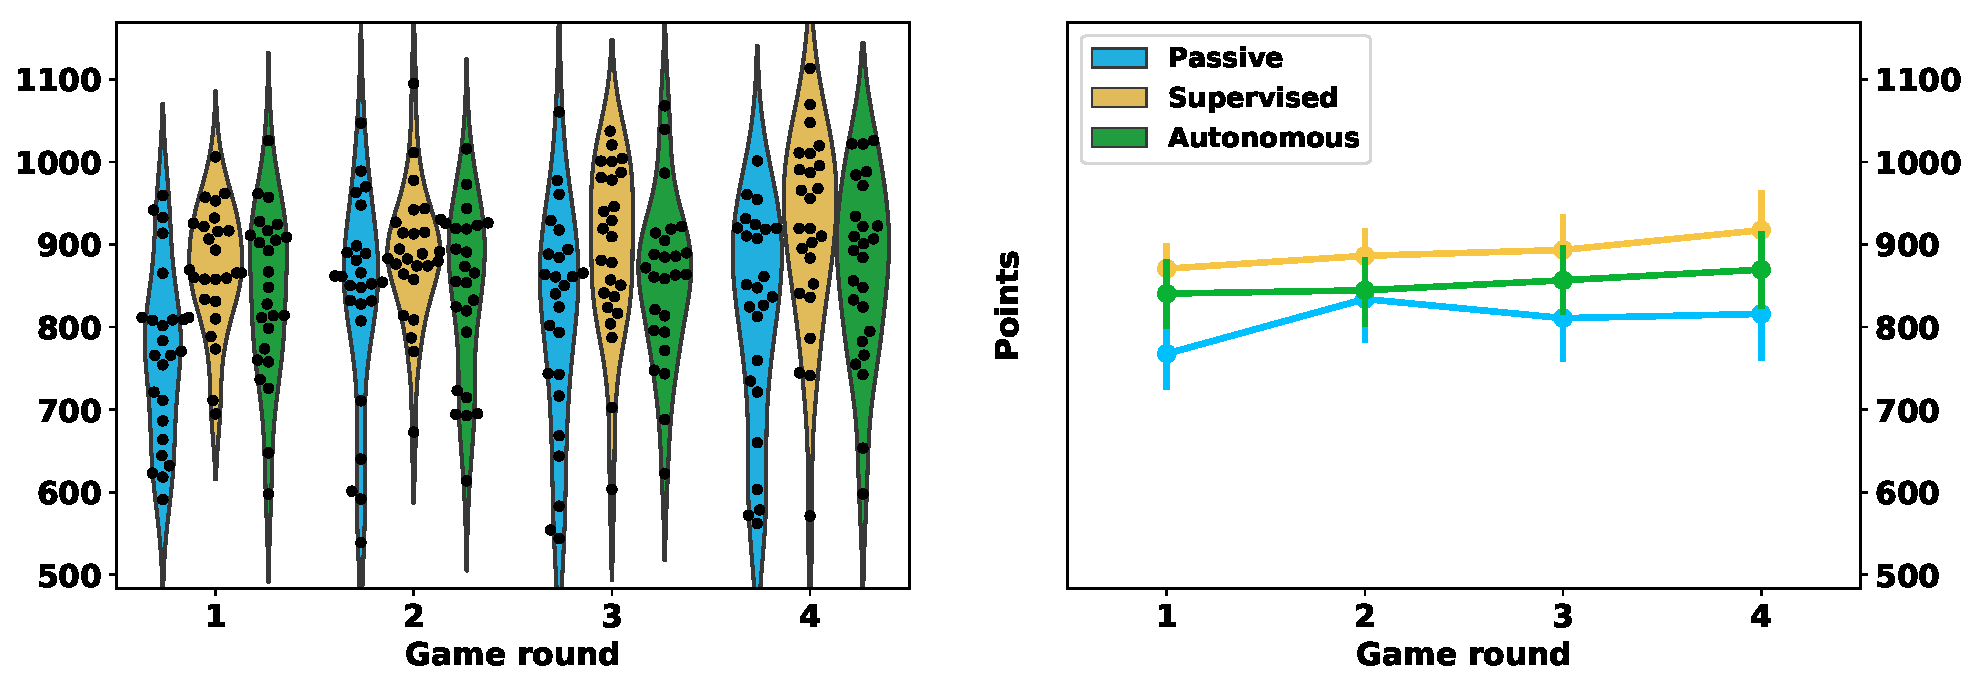
\includegraphics[width=1\linewidth]{points.pdf}
	\centering
	\caption{Points achieved by the children in each game session for the three conditions.}
	\label{fig:tutoring_points}
\end{figure}

\paragraph{Time}

Figure \ref{fig:tutoring_time} shows the evolution of interaction time across the four game sessions. A Bayesian mixed-ANOVA shows is inconclusive on the impact of the condition on the interaction time in the game ($B=1.1$). However, post-hoc tests show that there is no difference between the Supervised and the Autonomous conditions ($B=0.287$), whilst differences are observed between the Supervised and the Passive condition ($B=118$) and a tendency of difference between the Autonomous and the Passive conditions ($B=2.9$). This indicates that the Supervised robot allowed children to be better at the game, allowing them to maintain animal alive longer than a Passive robot. And the autonomous robot learn a policy tending to replicate this effect and without exhibiting differences with the supervised one.

\begin{figure}[ht]
	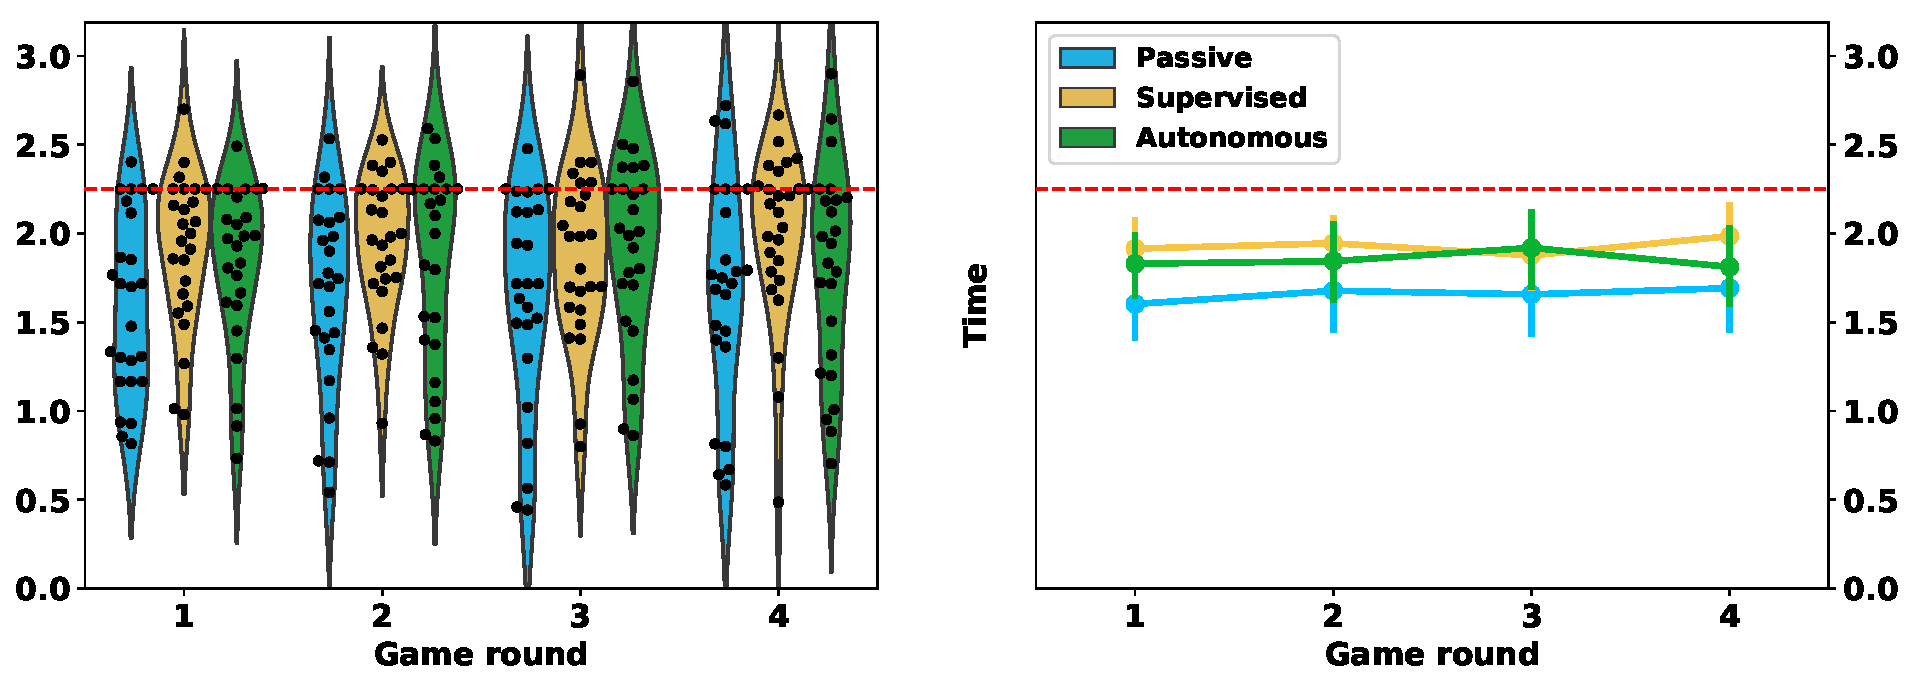
\includegraphics[width=1\linewidth]{time.pdf}
	\centering
	\caption{Interaction time for the four games for the three conditions.}
	\label{fig:tutoring_time}
\end{figure}


\paragraph{Summary}

These game metrics show that the action policy executed by the autonomous robot allows children to achieve similar results in the game than when the robot is supervised, and better results than when interacting with a passive robot. This provide support for H1 ("The robot reproduce the action policy demonstrated by the teacher enabling the child to achieve similar game metrics in autonomous and supervised condition but better than the passive condition"). 
%However, children learned similarly in the three conditions, so these improvements in the game did not transfer to improvements in the test neither for the Supervised robot nor the Autonomous one. This does not support H1 ("The robot support child learning: learning gain in passive condition $<$ learning gain in autonomous condition $<$ learning gain in supervised condition")

\subsection{Teaching the robot}
Figure \ref{fig:tutoring_supervision} presents the reaction of the teacher to the robot's suggestions across all the supervised sessions. In average the teacher accepted 22.3\% of all the proposition of the robot, which represented 35\% of all the actions executed by the robot and this effect tends to be stable across the sessions.

In post-hoc discussion, the teacher reported three phases in her teaching: 
\begin{itemize}
	\item First sessions: she was not paying much attention to the suggestions, mostly trying to have the robot executing a correct action policy.
	\item Session 5 to around 16: she was paying more attention to the suggestions without giving them much credit.
	\item Last sessions: she started to trust the robot more but without ever trusting it totally.
\end{itemize}

(I should add more about it...)

\begin{figure}[ht]
	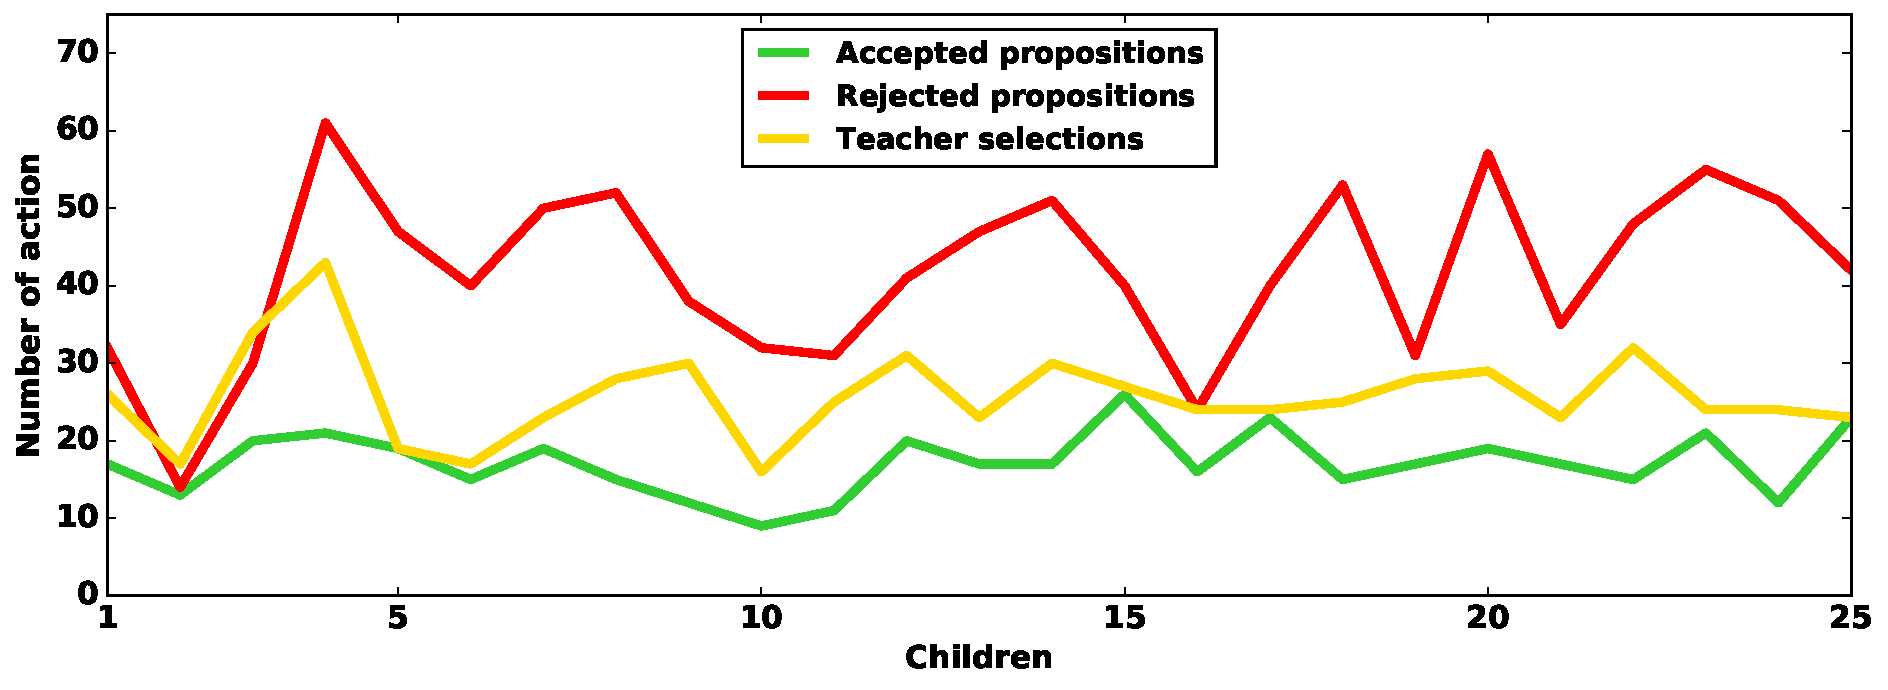
\includegraphics[width=1\linewidth]{./summary_supervision.pdf}
	\centering
	\caption{Summary of actions selection in the supervised condition: the `teacher selection' label represents each time the teacher manually selected an action for the robot to execute.}
	\label{fig:tutoring_supervision}
\end{figure}

The teacher did report a decrease of workload as she supervised the robot in more session. This is supported by behaviours such as typing on a laptop her observations, while gazing at the interface in multiple interactions (especially at the start of a session). However this decrease of workload seems to be due mostly to the teacher getting used to the interaction, and not to the online learning and improvement of the suggested proposition, this invalidate H3.
%Figure \ref{fig:tutoring_proposition} presents the reaction of the teacher to the robot's suggestions across all the supervised sessions. In average the teacher accepted 22.3\% of all the proposition of the robot (by enforcing the action, let it be executed or using the `Do it' button), which represents 35\% of the actions executed by the robot. This effect tends to be stable across the sessions. The teacher interaction pattern evolved overtime, such as by using mostly the `Cancel' button in the start then the `Skip' one, but in the end, the teacher used this two buttons mostly interchangeably even if the algorithm underlying reaction is different. Another observation is the evolution from using the auto-execution function to the `Do it' button once the teacher felt more comfortable in the supervision. The teacher reported three phases in her teaching: 
%
%\begin{itemize}
%	\item First sessions: she was not paying much attention to the suggestions, mostly trying to have the robot executing a correct action policy.
%	\item Session 20 to around 65: she was paying more attention to the suggestions without giving them much credit.
%	\item Last sessions: she started to trust the robot more but without ever trusting it totally.
%\end{itemize}
%
%\begin{figure}[ht]
%	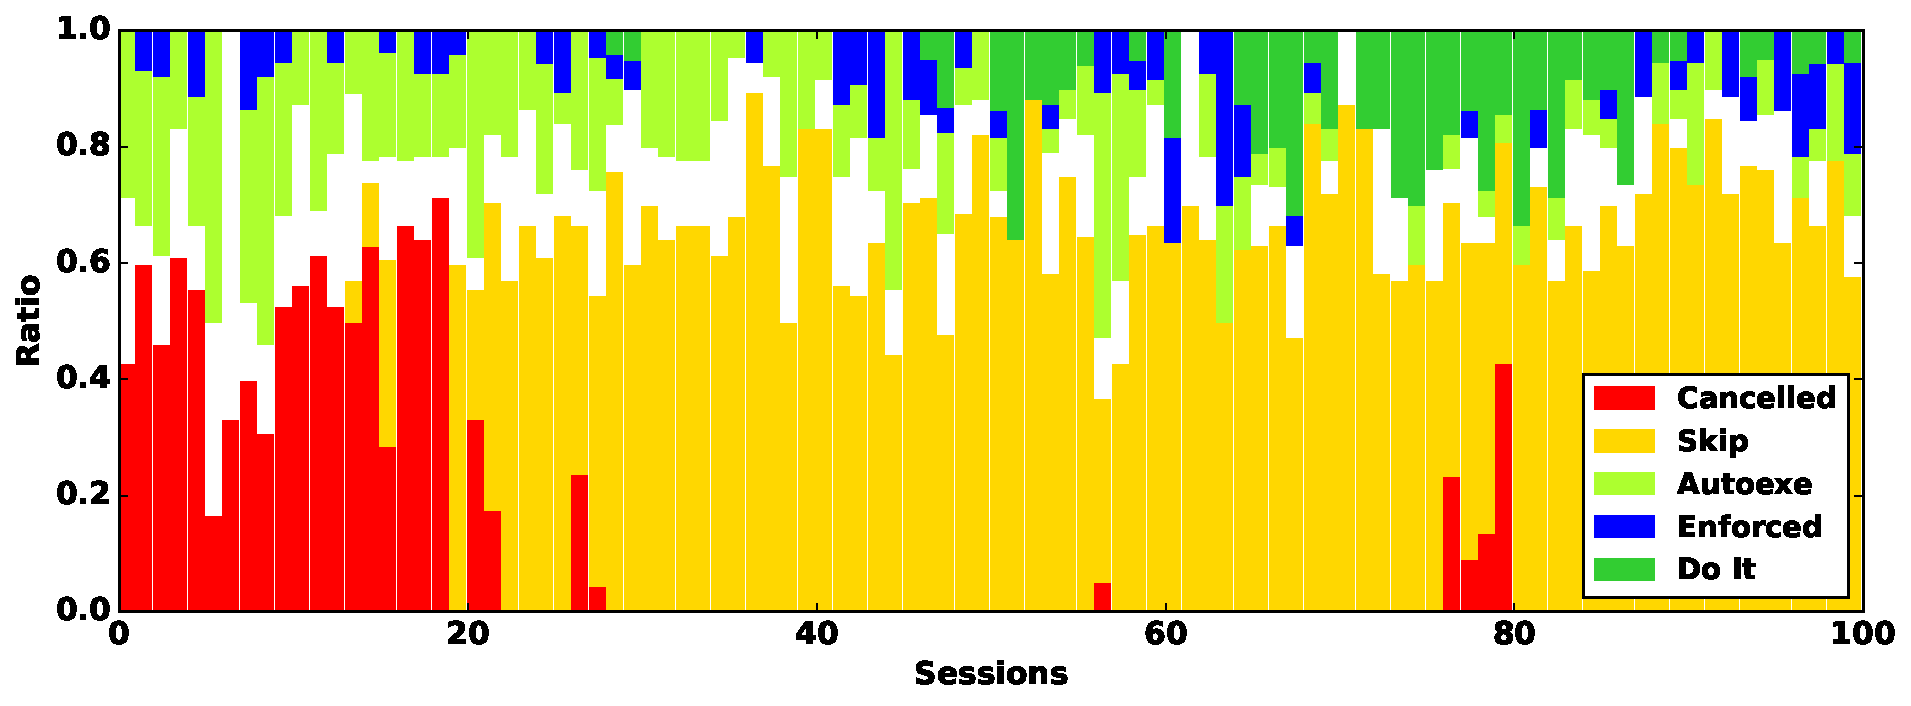
\includegraphics[width=1\linewidth]{propositions.pdf}
%	\centering
%	\caption{Teacher's reaction to the robot's propositions along the sessions.}
%	\label{fig:tutoring_proposition}
%\end{figure}
%
%
%\begin{figure}[ht]
%	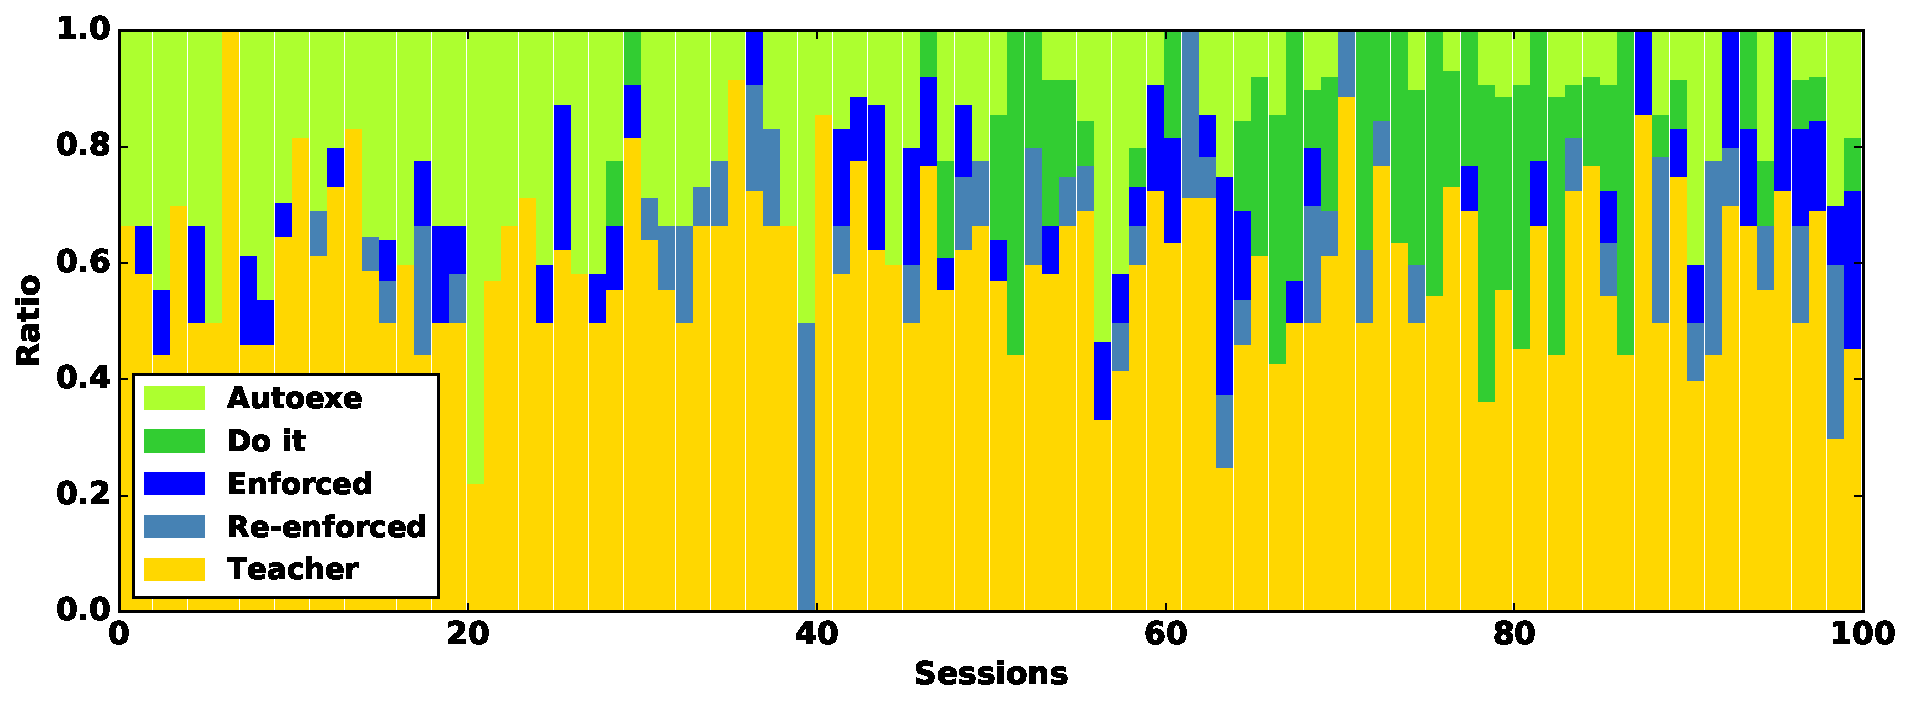
\includegraphics[width=1\linewidth]{selections.pdf}
%	\centering
%	\caption{Origin of the actions executed by the robot. Re-enforced actions indicates that an action has been selected after having been cancelled or skipped by the teacher.}
%	\label{fig:tutoring_selection}
%\end{figure}
%
%Additional comments:
%\begin{itemize}
%	\item The robot proposed in average 58\% more actions than the number of actions selected by the teacher.
%	\item As the time is continue and not discrete, the concept of correct actions is shifted, and actions selected by the teacher might have been proposed by the robot a fraction of second later without being counted as good proposition.
%	\item The teacher often cancelled/skip actions directly as they arrived without taking time to analyse them (limitation of this implementation of SPARC).
%	\item Evolution of teaching policy limits the potential of learning (not one single policy applied by the teacher, but an evolving one).
%	\item Children are different, so the teacher tried to apply different action policy for each child.
%\end{itemize}
%
%
%\begin{figure}[ht]
%	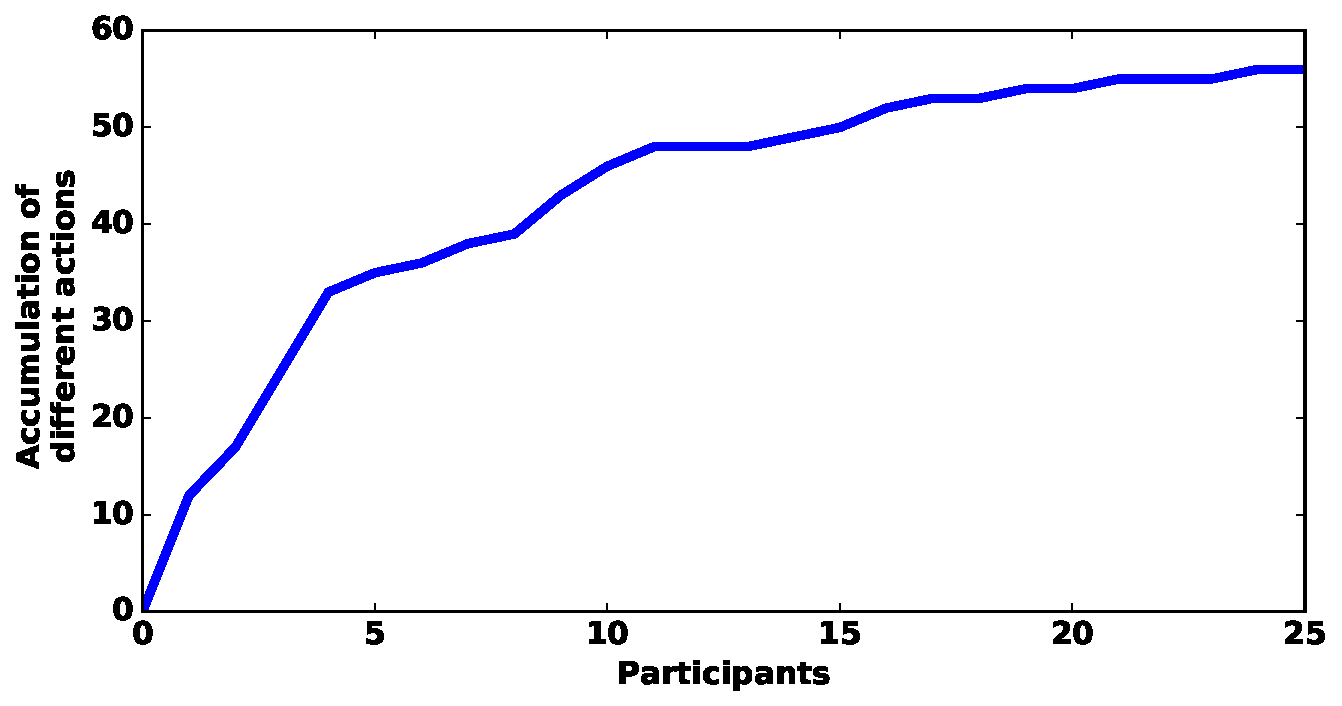
\includegraphics[width=.6\linewidth]{number_actions.pdf}
%	\centering
%	\caption{Accumulation of the number of different actions used by the teacher across the  participants.}
%	\label{fig:tutoring_actions}
%\end{figure}


\section{Discussion}

\subsection{Absence of effect of robot behaviour on learning gain}

\begin{itemize}
	\item Game self-exploratory, robot behaviour might distract the children
	\item Limits of the knowledge test: too open-ended, might have been better to have 10 random animals selected and ask the child to say yes/no?
	\item Limit of the performance calculation: the test was probably not able to capture the exact knowledge of children - Learning is about discovering interactions
\end{itemize}

\subsection{Absence of visible improvement of the robot}

\begin{itemize}
	\item The robot proposed in average 58\% more actions than the number of actions executed by the robot (approved and selected by the teacher): the threshold to select actions was probably too low, leading to too many propositions and the adaptivity of the threshold not good enough
	\item As the time is continuous and not discrete, the concept of correct actions is biased, there is no `correct' action policy associating an action to each time steps. Additionally the timing of the proposition was key as actions proposed just after a selection would have been discarded.
	\item To reduce the number of teacher selection, the robot would need to \emph{anticipate} every single teacher's action: not only knowing what action to do, but suggesting it the teacher before she started executing the action.
	\item The teacher often cancelled/skip actions directly as they arrived without taking time to analyse them (limitation of this implementation of SPARC).
	\item Evolution of teaching policy limits the potential of learning (not one single policy applied by the teacher, but an evolving one, including more actions as the teacher is more comfortable with the system).
	\item Children are different, so the teacher tried to apply different action policy for each child.
	\item Human centred interaction, the teacher was more focused on applying the best action policy for the child rather than teaching the robot.
	\item Application will always be human-centered, so the teaching of the robot will always be a side activity: actions that can hinder the robot learning will be taken if the child would profit for them.
	\item task complex
\end{itemize}

\subsection{Impact}
\begin{itemize}
	\item Complexity of the task
	\item discuss the supervision: not expert in machine learning, limited training
	\item Way to support that the autonomous robot was also able to sustain the engagement through the learning task
\end{itemize}

\subsection{Future work}
\begin{itemize}
	\item Potential for other applications?
	\item Ways to improve the study / How could the results have been better
\end{itemize}
\section{Summary}

